\documentclass{article}
\usepackage{amsmath, amssymb, tikz, geometry, graphicx, natbib, mwe, color, xcolor,
 listings, tabularx, pdfpages, blindtext, mathtools, stackengine, amsthm, pgfplots,bigints, relsize, upgreek, esint, array, multirow, schemata, wrapfig, cancel, comment}
\usepackage{hyperref}
\usepackage{slashed, enumitem}
\usepackage{titlesec}

\begin{comment}
code to write section, subsection and subsubsection title in a specific color
\titleformat{\section}
{\color{synthwave_text}\normalfont\Large\bfseries}
{\color{synthwave_text}\thesection}{1em}{} 

\titleformat{\subsection}
{\color{synthwave_text}\normalfont\large\bfseries}
{\color{synthwave_text}\thesubsection}{1em}{} 

\titleformat{\subsubsection}
{\color{synthwave_text}\normalfont\normalfont\bfseries}
{\color{synthwave_text}\thesubsubsection}{1em}{}
\end{comment}


\pgfplotsset{compat=1.9}

\colorlet{myWhite}{white!35!gray}
\definecolor{shadeofgray}{HTML}{181818}
\definecolor{shadeofviolet}{HTML}{0f022c}
\definecolor{synthwave_beckground}{HTML}{252334}
\definecolor{synthwave_text}{HTML}{e148aa}


\hypersetup{
    colorlinks=true,
    linkcolor=black,
    filecolor=magenta,      
    urlcolor=cyan,
    pdftitle={Elettotecnica},
    pdfpagemode=FullScreen,
}


\geometry{ 
 a4paper,
 left=10mm,
 right=10mm,
 top=10mm
 }
 
\lstdefinestyle{mystyle}{ 
bracketsstyle=\color{red}
}

\title{Elettrotecnica}
\author{Giuseppe Bumma}


% color option
%\pagecolor{synthwave_beckground} %{shadeofgray}
%\color{myWhite}

\renewcommand{\CancelColor}{\color{synthwave_text}}


\begin{document}

%Commands
\newcommand{\R}{\mathbb{R}}
\newcommand{\bb}[1]{\mathbb{#1}}
\newcommand{\cc}[1]{\mathcal{#1}}
\newcommand{ \lognormal }{\text{Lognormal} }
\newcommand{\tb}[1]{\textbf{#1}}
\newcommand*\circled[1]{\tikz[baseline=(char.base)]{%
            \node[shape=circle,draw,inner sep=2pt] (char) {#1};}}
%for using circled number in enumerate use:
%\begin{enumerate}[label=\protect\circled{\arabic*}]


\tableofcontents

\maketitle

\section{Introduzione}

\subsection{La carica elettrica e la forza di Coulomb}
Se due particelle cariche, supposte puntiformi, di carica $q_0$ e $q_1$, siano a una distanza finita fra loro nel vuoto, la \textbf{legge di Coulomb} descrive la forza elettrostatica interagente fra loro:
\[
    |F_C| \propto \frac{q_1q_2}{e^2}
\]
con $r$ distanza tra le due cariche.

\begin{center}
    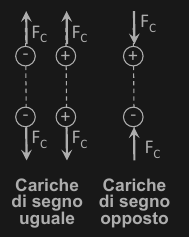
\includegraphics[scale=0.3]{Image/Forza di Coulomb.png}
\end{center}

La forza di Coulomb $F_C$ è diretta nella direzione di $r$. Quando $q_1$ e $q_2$ hanno lo
stesso segno la forza di Coulomb è repulsiva. Quando sono di segno opposto la
forza è attrattiva.\\
L'unità di misura, nel Sistema Internazionale (SI), della forza di Coulomb è il
newton [N] ed il coefficiente di proporzionalità è $1/(4\pi \epsilon_0)$ dove $\epsilon_0$ è la costante dielettrica del vuoto [$\epsilon_0 = 8,854x10^{-12} C^2/(Nm^2)$].
\vspace*{0.2cm}\\
L'unità di misura della carica elettrica nel sistema di misura SI è il \textbf{coulomb} [C]. La carica elementare nel SI è $e$ ove
\[
    e = 1,6021 x 10^{-19} C
\]
Protone ed elettrone hanno carica di valore assoluto e. Due protoni o
due elettroni si respingono. Un protone ed un elettrone si attraggono.
Per convenzione la carica del protone è positiva ($+e$) e quella dell'elettrone negativa (-$e$).\\
In natura esistano solamente cariche multiple di e. Non può esistere
una carica sottomultiplo di $e$.



\subsubsection{La cariche elettriche ed il loro moto}
Forza che agisce su una particella carica:
\[
    \vec F = q(\vec E + \vec u \times \vec B)
\]
\begin{align*}
    &\vec F: \text{forza [N]} &
    &\vec q: \text{carica elettrica [C]} &
    &\vec u: \text{velocità della carica [m/s]}
\end{align*}
\begin{align*}
    &\vec E: \text{campo elettrico} &
    &\vec B: \text{vettore induzione magnetica}
\end{align*}
\begin{itemize}
    \item Se $\vec B=0$ si ha la cosiddetta \textbf{Forza elettrostatica}
    \[
        \vec F = q \vec E
    \]
    Quindi il campo elettrico $\vec E = \frac{\vec F}{q} $ è una forza per unità di carica [N/C].
    \vspace*{0.1cm}\\
    Campo elettrico e forza elettrostatica da cui esso deriva hanno la stessa
    direzione. Perciò il campo produce un'accelerazione della carica lungo la
    propria direzione.
    \vspace*{0.1cm}\\
    Nel SI l'unità di misura di $\vec E$ è: $N/C = V/ m = m \ kg \ s^{-2} C^{-1}$.
    \vspace*{0.2cm}\\
    \item Se $\vec E=0$ si ha la \textbf{Forza di Lorentz}
    \[
        \vec F = q(\vec u \times \vec B)
    \]
    Quindi il vettore induzione magnetica $\vec B$ è una forza per unità di carica e di velocità [$N s / C m$].
    Campo elettrico e forza elettrostatica da cui esso deriva hanno la stessa
    direzione. Perciò il campo produce un'accelerazione della carica lungo la
    propria direzione.
    Nel SI l'unità di misura di $\vec E$ è: $N/C = V/ m = m \cdot kg \cdot s^{-2} \cdot C^{-1}$.
\end{itemize}
Una particella carica induce una forza sulle cariche
che la circondano. Tale forza può essere attrattiva o
repulsiva. Essa è la forza Coulombiana $F_C$ (o forza
elettrostatica). In ogni punto della regione attorno
alla carica o in presenza ad una distribuzione di
cariche vi è un campo elettrico $\vec E(x,y,z)$ definito dalla
forza indotta su una carica di prova puntiforme
unitaria posta nel punto considerato.
\begin{center}
    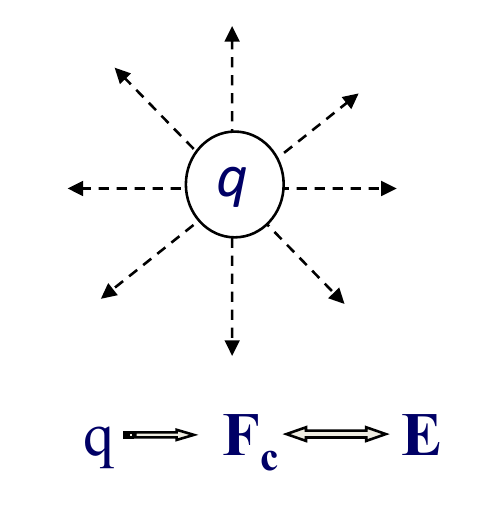
\includegraphics[scale=0.27]{Image/Forza elettrostatica.png}
\end{center}
Qualora su una carica in moto si induca una forza
deviante perpendicolare al moto, tale forza è la
forza magnetica o forza di Lorentz 
$F_L$. Il campo
di induzione magnetica $\vec B(x,y,z)$, legato a $\vec F_L$, è
dato dalla forza indotta su una carica unitaria in
moto per unità di velocità della carica stessa. La
direzione del campo $\vec B$ è perpendicolare alla
velocità ed alla forza $\vec FL$ . Il campo $\vec B$ è
perpendicolare alla velocità della carica ed alla
forza indotta.

\subsection{Densità volumetrica di carica}
La carica elettrica non può essere creata o distrutta (legge della
conservazione della carica elettrica). Può solo essere trasferita. Pertanto, la
carica elettrica totale di un sistema isolato non può variare.\\
La densità volumetrica di carica (o distribuzione di carica) è definita da:
\[
    \rho_C (x,y,z) = \lim_{\Delta t \rightarrow 0} \frac{\Delta q}{\Delta \tau} = \frac{dt}{dq}  
\]
dove $d \tau$ è l'elemento infinitesimo di volume.

\subsubsection{Densità di corrente \texorpdfstring{$J$}{J}}
La densità di corrente elettrica $\vec J$ è il vettore il cui modulo è la quantità di
carica che attraversa una superficie unitaria perpendicolare alla velocità $\vec u$
delle cariche. La direzione ed il verso di $\vec J$ sono la direzione ed il verso di $\vec u$:
\[
    \vec J \cdot \hat n = \lim_{\Delta S \rightarrow 0} \lim_{\Delta t \rightarrow 0} \frac{\Delta Q}{\Delta S \Delta t}
\]
$\vec J$: densità di corrente $\left[\frac{C}{m^2\cdot s}\right] = \left[\frac{A}{m^2} \right]$

\begin{center}
    \includegraphics[scale=0.3]{Image/Densità di corrente.png}
\end{center}

$\vec J(x,y,z)$ definisce un campo vettoriale ed è la densità di flusso delle
cariche. La corrente elettrica $i$ è il flusso di carica attraverso una
superficie $S$:
\[
    i = \iint\limits_S \vec J \cdot \hat n \ dS
\]




\subsection{Corrente elettrica}
La corrente elettrica i che attraversa una superficie è la quantità di carica
che attraversa la superficie nell’unità di tempo:
\[
     i = \frac{\Delta q}{\Delta t} 
\]
Se si considera un cavo conduttore, ad esempio, la corrente nel conduttore è la
quantità di carica che attraversa una sezione del cavo nell'unità di tempo.

\begin{center}
    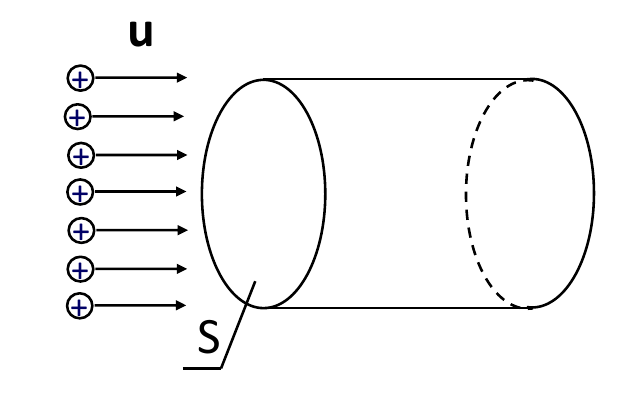
\includegraphics[scale=0.3]{Image/Corrente conduttore.png}
\end{center}

L'unità di misura SI è l'ampere [$A$] dove $A = \frac{C}{s}$
\vspace*{0.1cm}\\
La \textbf{corrente elettrica istantanea} è:
\[
    i(t) = \lim_{\Delta t \rightarrow 0} \frac{\Delta q}{\Delta t} = \frac{dq}{dt}
\]



\subsection{Tensione elettrica e differenza di potenziale elettrico}
La \textit{tensione elettrica} $e_{12}$ fra i punti 1 e 2 lungo il
percorso $l$, è il lavoro $L^{1\rightarrow 2,l}_{q=1}$ che il campo elettrico
$\vec E(x,y,z)$ compie per portare una carica unitaria dl
punto 1 al punto 2 lungo $l$:
\[
    e_{12} = \int_{1,l}^2 \vec E \cdot d \vec l
\]

\begin{center}
    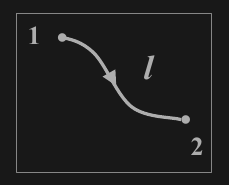
\includegraphics[scale=0.3]{Image/Tensione.png}
\end{center}

Per spostare la carica $q$ dal punto 1 al 2 il lavoro è:
\[
    L^{1 \rightarrow 2,l}_q = q \cdot e_{12}
\]
L'unità di misura SI di $e_{12}$ è il volt [$V$] dove $V = \frac{J}{C} = m^2 \cdot kg \cdot s^{-2} \cdot C^{-1}$.
Qualora la tensione e 12 dipenda dai valori di una
funzione $v(x,y,z)$ definita in una regione che contiene la linea $l$ essa diviene:
\[
    e_{12} = \int_{1,l}^{2}\vec E \ d\vec l = - \int_{1,l}^{2} dv = v_1 - v_2 = v_{12}
\]
dove $v(x,y,z)$ è la \textbf{funzione potenziale elettrico} e $v_{12}$
è la \textbf{differenza di potenziale elettrico}.
\vspace*{0.1cm}\\
Poiché $v_{12}$ è la differenza fra i valori che la funzione $v(x,y,z)$ assume nel punto
iniziale e nel punto finale di $l$, $v_{12}$ non dipende dal percorso che unisce i due
punti. Quindi il campo $\vec E$ è un \textbf{vettore conservativo} \footnote{un campo conservativo è un campo il cui integrale lineare è indipendente dalla traiettoria} con $\vec E = \vec \nabla \cdot v(x,y,z)$.
\vspace*{0.1cm}\\
Per un percorso chiuso $l_c$ contenuto nella regione ove $\vec E$ è conservativo, si ha:
\[
    e_l = \oint _{l_c} \vec E \cdot d \vec l_c = - \oint _{l_c} \vec \nabla \cdot v  \ d\vec l_c = 0
\]



\subsection{Legge di Ampere-Prima legge di Maxwell}
La grandezza vettoriale campo magnetico H è definito dalla legge di Ampere (prima legge di Maxwell)
\[
    \oint _{l_c} \vec H \ d \vec l_c = i_t
\]
dove la corrente totale $i_t = i + i_s$.\\
In questo caso la corrente totale $i_t$ è il flusso del vettore $J_t$ i ovunque solenoidale ($J_t = J + \partial D/ \partial t$). Perciò $i_t$ è il flusso concatenato con la linea chiusa $l_C$ contorno della superficie che attraversa. Il verso di percorrenza di $l$ è determinato con regola della vite destrogira.
\begin{center}
    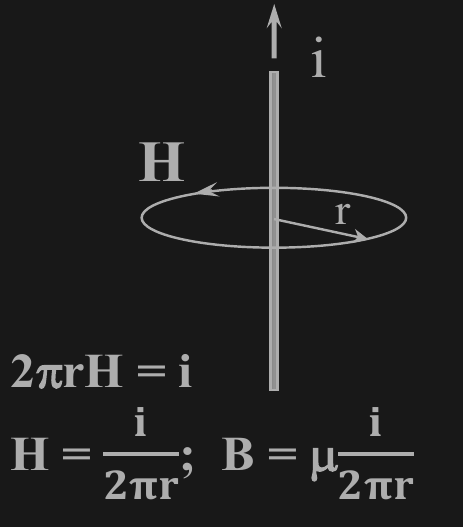
\includegraphics[scale=0.3]{Image/Campo magnetico.png}
    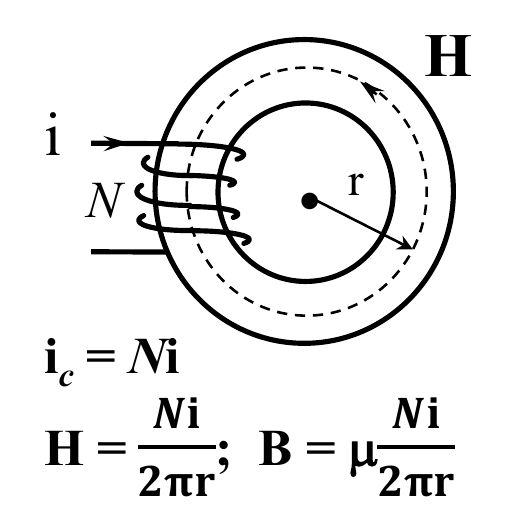
\includegraphics[scale=0.3]{Image/Campo magnetico-2.png}
\end{center}
L'unità di misura SI di $\vec H$ è l'ampere su metro [$\frac{A}{m}$].
Per materiali lineari: $\vec B = \mu \vec H$ ove $mu$ è la permeabilità magnetica del materiale. Per mezzi non lineari
$\vec B = f(\vec H)$. Solitamente per i materiali magnetici non lineari $f$ è una funzione \textbf{isteretica} (materiali
ferromagnetici).
\begin{align*}
    \oint_{l_C}\vec H \ d \vec l &= \iint\limits_{S} \left( \vec J + \frac{\partial
    D}{\partial t} \right) \ \hat n \ dS\\
    &= \underbrace{\iint\limits_{S} \vec J \ \hat n \ dS}_{\text{corrente di conduzione } I} + \underbrace{\iint\limits_{S} \frac{\partial D}{\partial t} \ \hat n \ dS}_{\iint\limits_{S} \partial D \ \hat n \ dS =\vec \Phi(D)} =\\
    &= I + \underbrace{\frac{\partial \vec \Phi(D)}{\partial t}}_{\text{corrente di spostamento}}
\end{align*}
Immaginiamo di descrivere due superfici $S_1$ e $S_2$ sulla linea chiusa $l_C$
\[
    \oint_{l_C} \vec H \ d\vec l = \iint\limits_{S_1}\left( \vec J + \frac{\partial D}{\partial t} \right) \hat n_1 \ dS_1 = \iint\limits_{S_2}\left( \vec J + \frac{\partial D}{\partial t} \right) \hat n_2 \ dS_2
\]
Prendiamo una superficie chiusa $S_C$ su $S_2$, allora
\[
    \oint_{S_C}\underbrace{\bigg( \vec J + \frac{\partial D}{\partial t}\bigg)}_{\text{vettore solenoidale}}\hat n_C \ dS_C = \iint\limits_{S_2}\left( \vec J + \frac{\partial D}{\partial t} \right) \hat n_2 \ dS_2 - \iint\limits_{S_1}\left( \vec J + \frac{\partial D}{\partial t} \right) \hat n_1 \ dS_1 = 0
\]



\subsection{Legge dell'induzione di Faraday-Seconda legge di Maxwell}
La legge dell'induzione (o legge di Faraday
od anche seconda legge di Maxwell)
stabilisce che:
\[
    e_{l_C} = \oint_{l_C}
    \vec E \ d\vec l_C = -\frac{d \Phi}{dt}
\]
\begin{center}
    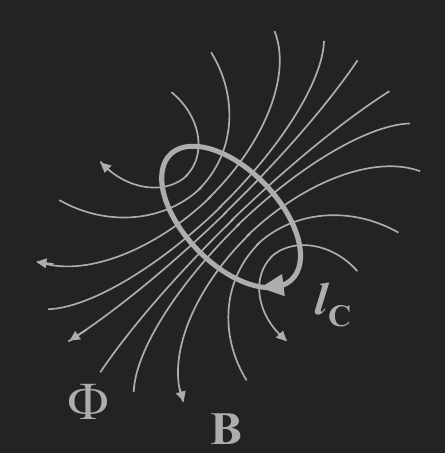
\includegraphics[scale=0.3]{Image/Legge di Faraday.png}
\end{center}
ove $\Phi$ è il flusso magnetico concatenato con
la linea chiusa $l_c$. (direzione di $l_C$ data dalla
regola della vite destrogira).\\
$e_{l_c}$ è la tensione elettrica indotta sulla
linea chiusa dalla variazione del flusso
magnetico concatenato con $l_c$; essa è detta
\textbf{forza elettromotrice} (f.e.m.).
\vspace*{0.1cm}\\
\textbf{N.B.} In questo caso $\vec E$ non à conservativo.



\subsection{Conservazione della carica elettrica}
La carica elettrica non si crea né si distrugge. Perciò la diminuzione della carica elettrica
all'interno di un volume $\tau$ corrisponde alle
cariche che lasciano $\tau$ fluendo attraverso la
superficie chiusa $S$, superficie esterna di $\tau$.
\begin{center}
    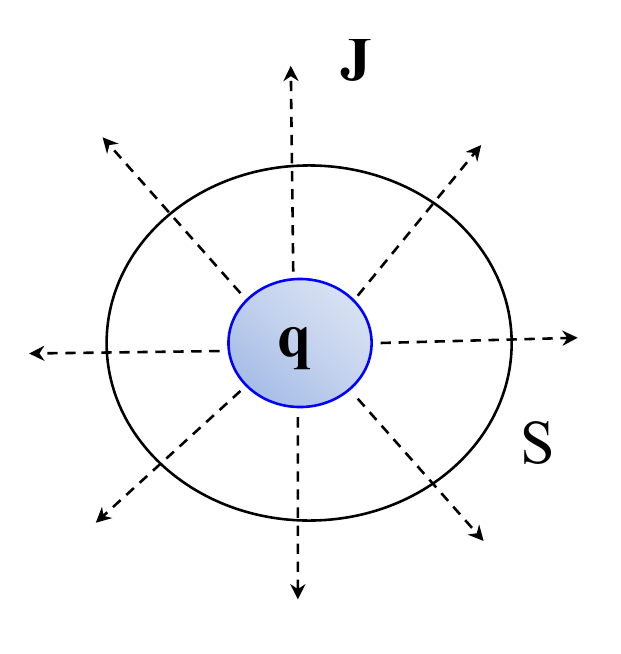
\includegraphics[scale=0.3]{Image/Conservazione della carica.png}
\end{center}
La \textbf{\textit{
legge di conservazione della carica elettrica}} afferma questo ed è espressa
dall'espressione: 
\[
    \oiint_{S} \vec J \ \hat n \ dS = - \frac{dQ}{dt}
\]
si ha variazione di cariche solo se c'è passaggio di corrente.




\subsection{Legge di Gauss}
Il campo di induzione elettrica o campo spostamento elettrico è definito dalla
legge di Gauss.
Considerando una superficie chiusa $S$,
che delimita il volume $V$; sia $\hat n$ il versore
normale alla superficie. La legge di Gauss
afferma che:
\[
    \oiint_{S} \vec D \ \hat n \ dS = \iiint_{V}\rho \ dV = Q
\]



\subsection{Forza elettromotrice}
$\vec E$ e $\vec B$ descrivono le forze prodotte dal fenomeno elettromagnetico sulle
cariche (forza elettrica per unità di carica e forza magnetica per unità di
carica e di velocità della carica). Esse descrivono ciò che viene prodotto dal
fenomeno EM. Ne descrivono l'\textbf{effetto}.
\vspace*{0.1cm}\\
$\vec D$ ed $\vec H$ descrivono ciò che produce il fenomeno EM (la carica elettrica nel
primo caso e la corrente totale nel secondo). Ne descrivono la \textbf{causa}.

\subsection{Leggi dell'Elettromagnetismo in forma integrale}
\renewcommand{\arraystretch}{2.5}
\begin{center}
    \begin{tabular}{|c|c|}
        \hline
        $\oint_{l_c} \vec H \ d \vec l_c = i_t$ & $1^o$ legge di Maxwell\\
        \hline 
        $\oint_{l_c} \vec E \ d \vec l_c = \dfrac{d\Phi}{dt}$ & $2^o$ legge di Maxwell\\
        \hline
        $\oiint \vec J \ \hat n dS = - \dfrac{dq}{dt}$ & legge di conservazione della carica \\
        \hline
        $\oiint \vec D \ \hat n dS = q $ & legge di Gauss\\
        \hline 
        $\oiint \vec J_t \ \hat n dS = 0 $ & $\vec Jt$ ovunque solenoidale\\
        \hline t
        $\oiint _S \vec B \ \hat n dS=0$ & $\vec B$ ovunque solenoidale\\
        \hline
    \end{tabular}    
\end{center}
Tre di queste sei equazioni sono linearmente indipendenti, le altre tre si ottengono dalle prime tre.



\subsection{Leggi dell'Elettromagnetismo in forma locale}
\begin{center}
    \begin{tabular}{|c|c|}
        \hline
        $\nabla \times \vec H = \vec J + \dfrac{\partial
        \vec D}{\partial t}$ & 1° legge di Maxwell (dal teorema di Stokes) \\
        \hline 
        $\nabla \times \vec E = - \dfrac{\partial
        \vec B}{\partial t}$ & 2° legge di Maxwell
        (dal teorema di Stokes)\\
        \hline
        $\nabla \cdot \vec J = - \dfrac{\partial \rho_c}{\partial t} $ & legge di conservazione della carica (teor. divergenza)\\
        \hline
        $\nabla \cdot \vec D = \rho_c$ & legge di Gauss (dal teorema della divergenza)\\
        \hline
        $\nabla \cdot \vec J_t = 0$ & $\vec J_t$ ovunque solenoidale (dal teorema della divergenza)\\
        \hline 
        $\nabla \cdot \vec B =0$ & $\vec B$ ovunque solenoidale (dal teorema della divergenza)\\
        \hline
    \end{tabular}    
\end{center}
Tre di queste sei equazioni sono linearmente indipendenti, le altre tre si ottengono dalle prime tre.



\subsection{Relazioni materiale}
$\vec E$ e D, $\vec B$  ed $\vec H$  descrivono i fenomeni dell'EM in modo diverso. $\vec E$ e $\vec D$ si
riferiscono al fenomeno Elettrico, $\vec B$  ed $\vec H$  al fenomeno magnetico. $\vec D$ ed $\vec H$ 
descrivono i due fenomeni misurando ciò che li origina: la carica il primo, ed il
moto della carica il secondo. Gli effetti misurati da $\vec E$ e da $\vec B$  sono in entrambe i
casi le forze indotte. Essi dipendono da come i diversi materiali reagiscono.
Inoltre, dipendentemente dalla proprietà del materiale, ad un certo valore del
campo $\vec E$ si induce un determinato moto di carica misurato da $\vec J$ . Le relazioni
fra queste descrizioni spesso sono lineari. A volte però non lo sono con
relazioni anche di tipo isteretico.
\begin{center}
    \begin{tabular}{|c|c|}
    \hline
    \textbf{Materiali lineari} & \textbf{Materiali non lineari}\\
    \hline 
    $\vec D = \epsilon \vec E$ & $\vec D = f_1(\vec E)$\\
    \hline 
    $\vec B = \mu \vec H$ & $\vec B = f_2(\vec H)$\\
    \hline 
    $\vec J = \sigma \vec E$ & $\vec J = f_3(\vec E)$\\
    \hline
\end{tabular}
\end{center}
con $\epsilon$ costante dielettrica, $\mu$ permeabilità magnetica e $\sigma$ conducibilità termica.
\vspace*{0.1cm}\\
la costante dielettrica (permittività elettrica) $\epsilon$, e la permeabilità magnetica $\mu$
di un materiale sono espresse per mezzo dei loro valori relativi $\epsilon_r$ ed $\mu_r$ in riferimento al loro valore nel vuoto $\epsilon_0$ ed $\mu_0$:
\begin{align*}
    &\epsilon = \epsilon_r \epsilon_0 &\text{dove } \epsilon_0 = 8,856 x 10^{-12} Farad/metro \left[\frac{F}{m}\right]\\
    &\mu = \mu_r \mu_0 &\text{dove } \mu_0 = 1,256 x 10^{-6} Henry/metro \left[\frac{H}{m}\right]
\end{align*}
Riporto alcuni valori di $\epsilon_r$
\begin{center}
    \renewcommand{\arraystretch}{1}
    \begin{tabular}{c|c}
         & $\epsilon_r$\\
        \hline
        vuoto & 1\\
        aria & $\simeq 1$\\
        plastica & 2-5\\
        vetro & 4-8\\
        acqua & 80
    \end{tabular}
\end{center}
Molto diverse sono le variazioni per materiali differenti della
conducibilità elettrica, della permeabilità magnetica e della costante
dielettrica.
Per la conducibilità elettrica $\sigma$ vi è una variazione anche di $10^{23}$ (23 ordini
di grandezza) fra materiali isolanti e materiali conduttori.
Per la permeabilità magnetica $\mu$ la variazione raggiunge al massimo un
valore di circa $10^5$ (5 ordini di grandezza).
Per la costante dielettrica $\epsilon$ la variazione massima si riduce ad un valore
massimo di circa $10^3$ (3 ordini di grandezza).
\vspace*{0.2cm}\\
La relazione fra $\vec J$ ed $\vec E$ è
anche definita dalla
resistività elettrica $\rho$:
\[
    \vec E = \rho \vec J
\]
dove
$\rho = \frac{1}{\sigma}$
$\sigma$ è in Siemens/metro [$\frac{S}{M}$] e $\rho$ in Ohm/metro [$\frac{\Omega}{m}$].


\subsection{SI Units}
\subsubsection{Unità derivate SI}

    \begin{tabular}{|m{35mm}|c|c|m{35mm}|}
    \hline
    Grandezza&
    Simbolo (nome)&
    Unità SI non di base&
    Unità SI di base\\
    \hline 
    Carica elettrica&
    $C$ (Coulomb)&
    & 
    $s \times A$\\
    \hline
    Tensione elettrica e differenza di potenziale elettrico &
    $V$ (Volt)&
    $ \dfrac{W}{A}$&
    $m^2 \times kg \times s^{-3} \times A^{-1}$\\
    \hline
    Forza&
 $N$ (Newton)&
 &
 $m \times kg \times s^{-2}$\\
 \hline
Energia/Lavoro&
 $J$ (Joule)&
 $N \times m$&
 $m^2 \times kg \times s^{-2}$\\
 \hline
Potenza&
 $W$ (Watt)&
 $\dfrac{J}{s}$&
 $m^2 \times kg \times s^{-3}$\\
 \hline 
Flusso magnetico&
 $Wb$ (Weber)&
 $V \times s$&
 $m2 \times kg \times s-2 \times A^{-1}$\\
 \hline 
Induzione magnetica&
 $T$ (Tesla)&
 $\dfrac{Wb}{m^2}$&
 $kg \times s^{-2} \times A^{-1}$\\
 \hline 
Resistenza elettrica&
 $\Omega$ (Ohm)&
 $\dfrac{V}{A}$&
 $m^2 \times kg \times s^{-3} \times A^{-2}$\\
 \hline 
Conduttanza elettrica&
 $S$ (Siemens)&
 $\dfrac{A}{V}$&
 $m^{-2} \times kg^{-1} \times s^3 \times A^2$\\
 \hline 
Capacità&
 $F$ (Farad)&
 $\dfrac{C}{V}$&
 $m^{-2} \times kg^{-1} \times s^4 \times A^2$\\
 \hline 
Induttanza&
 $H$ (Henry)&
 $\dfrac{Wb}{A}$&
 $m^2 \times kg \times s^{-2} \times A^{-2}$\\
 \hline
Frequenza&
 $Hz$ (Hertz)&
 &
 $s^{-1}$\\
 \hline 
\end{tabular}


\subsubsection{Prefissi SI}
\begin{center}
    \renewcommand{\arraystretch}{1.5}
    \begin{tabular}{|c|c|c|}
        \hline
        Factor & Name & Symbol\\
        \hline 
        $10^{-24}$ & yocto  & y\\
        \hline 
        $10^{-21}$ & zepto & z\\
        \hline 
        $10^{-18}$ & atto & a\\
        \hline 
        $10^{-15}$ & femto & f\\
        \hline 
        $10^{-12}$ & pico & p\\
        \hline 
        $10^{-9}$ & nano & n\\
        \hline 
        $10^{-6}$ & micro & $\mu$\\
        \hline 
        $10^{-3}$ & milli & m\\
        \hline 
        $10^{-2}$ & centi & c\\
        \hline 
        $10^{-1}$ & deci & d\\
        \hline 
        $10^{1}$ & deca & da\\
        \hline 
        $10^{2}$ & hecto & mh\\
        \hline 
        $10^{6}$ & mega & M\\
        \hline 
        $10^{9}$ & giga & G\\
        \hline 
        $10^{12}$ & tera & T\\
        \hline 
        $10^{15}$ & peta & P\\
        \hline 
        $10^{18}$ & exa & E\\
        \hline 
        $10^{21}$ & zetta & Z\\
        \hline 
        $10^{24}$ & yotta & Y\\
        \hline 
    \end{tabular}
\end{center}






\section{Circuiti elettrici}
\subsection{Introduzione}
I circuiti elettrici sono degli elementi interconnessi tra loro e le connessioni possono essere considerate dei conduttori ideali.
\vspace*{0.2cm}\\
\textbf{Ipotesi:}
\begin{itemize}
    \item $ \dfrac{\partial \vec B}{\partial t} = 0 $ o $ \dfrac{\partial \vec D}{\partial t} = 0 $
    \item $L_c << \lambda$ (lunghezza d'onda)
\end{itemize}
Ricordiamo che $\lambda = \dfrac{c}{f} = \left[ \dfrac{velocita \ onda}{frequenza \ onda} \right]$.
\subsubsection*{Esempio}
La rete elettrica ha frequenza $f = 50 Hz$
\[
    \lambda = \dfrac{c}{f} = \dfrac{3 \cdot 10^{8}}{50} \simeq 6000 km
\]
infatti la linea di trasmissione della corrente elettrica è $L_c = 10^3 km$.
\vspace*{0.2cm}\\
Gli elementi del circuito vengono chiamati \textit{multipoli}; di seguito si riporta la lista:
\begin{itemize}
    \item Nodo: punto di intersezione tra 2 o più elementi;
    \item Maglia: linea chiusa all'interno del circuito;
    \item Ramo: componenti insieme ai suoi morsetti
\end{itemize}
Le formule fondamentali per i circuiti sono:
\begin{align*}
    &\underbrace{P(t) = v(t) \cdot i(t)}_{\text{potenza}} & &\underbrace{W(t) = \int P(t) \ dt}_{\text{energia}}
\end{align*}
Per ogni circuito esistono due convenzioni per il verso della corrente
\begin{center}
    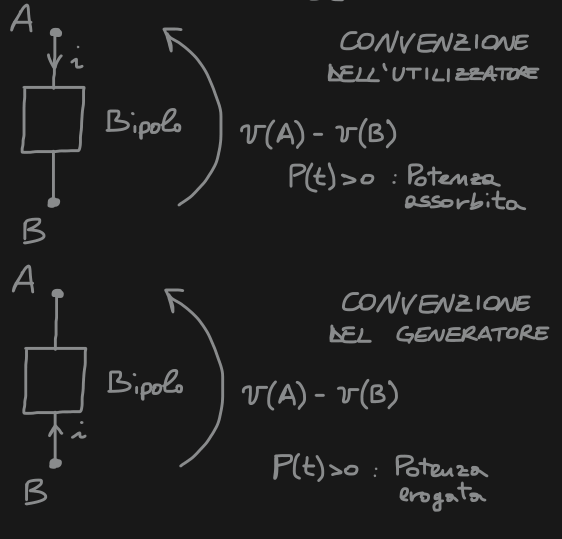
\includegraphics[scale=0.3]{Image/Convenzione.png}
\end{center}
Ad esempio, nel caso di una batteria ricaricabile, se si utilizza la convenzione del generatore:
\begin{align*}
    &\text{Scarica} & v&=1,5 V & i&=1A & P&=v\cdot i = 1,5W \ {\color{violet}>0}\\
    &\text{Carica} & v&=1,5 V & i&=-1A & P&=v\cdot i = -1,5W \ {\color{violet}<0}
\end{align*} 
mentre se si utilizza la convenzione dell'utilizzatore i segni di corrente e ,propedeuticamente, di potenza sono invertiti 
\begin{align*}
    &\text{Scarica} & v&=1,5 V & i&=-1A & P&=v\cdot i = -1,5W \ {\color{violet}<0}\\
    &\text{Carica} & v&=1,5 V & i&=1A & P&=v\cdot i = 1,5W \ {\color{violet}>0}
\end{align*} 


\subsection{Risolvere un circuito}
Risolvere un circuito vuol dire calcolare le tensioni e le correnti di tutti i componenti.
\subsubsection{Prima legge (LKT)}
Usando le \textbf{leggi di Kirchhoff} e le \textbf{leggi costitutive}
\[
    \oint \vec E \ d \vec l = \oiint \dfrac{\partial \vec B}{\partial t}\ \hat n dS \underbrace{=}_{Hp.1} 0
\]
ne consegue che il campo elettrico è conservativo e dunque si può definire una differenza di potenziale.
\[
    \int_l \vec E \ d \vec l = v(A) - v(B) = v_{AB}
\]
\begin{align*}
    \underbrace{\oint \vec E \ d \vec l}_{0} &= \int_{A}^{B} \vec E \ d\vec l + \int_{B}^{C} \vec E \ d\vec l + \int_{C}^{A} \vec E \ d\vec l \\
    &= v_{BA}+ v_{CB} + v_{AC} \\
    &= 0
\end{align*}
da qui la $1^a$ legge di Kirchhoff per le tensioni:
\[
    \sum_{k=1}^nv_k=0
\]
nella singola maglia.


\subsubsection*{Esempio}
\begin{center}
    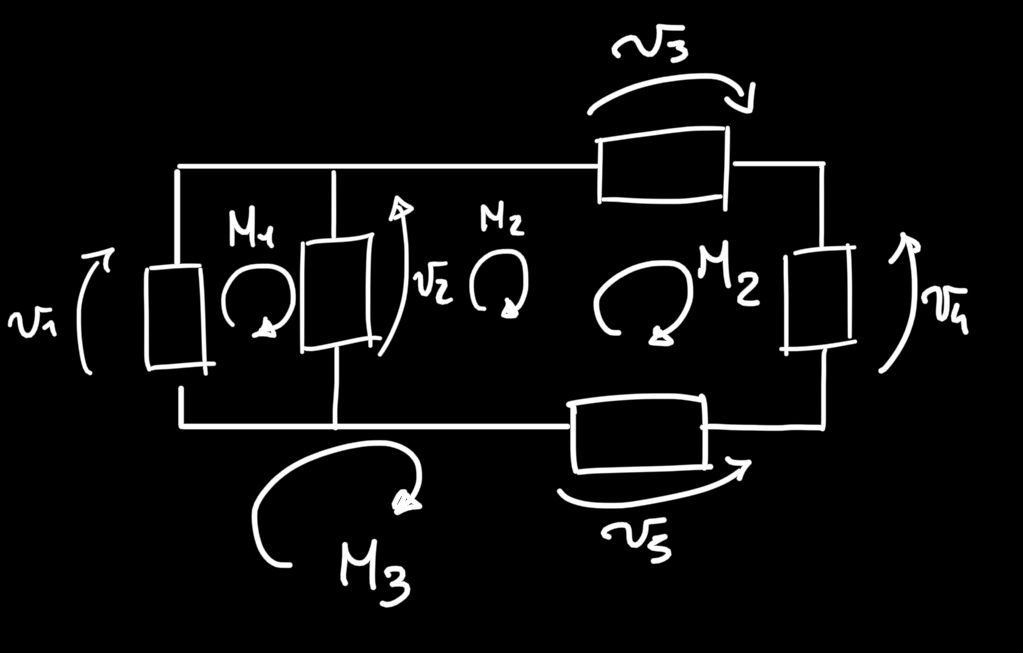
\includegraphics[scale=0.37]{Image/Esempio1-Circuiiti.png}
\end{center}
\[
\begin{cases}
    M_1: & v_1 - v_2 = 0\\
    M_2: & v_2+v_3-v_4-v_5 = 0\\
    M_3: & v_1 + v_3 - v_4 - v_5=0
\end{cases}
\]
I versi delle differenze di potenziale sono date dal testo dell'esercizio, il verso di percorrenza
della maglia è scelto arbitrariamente. Il segno positivo o negativo delle tensioni è determinato in base al verso di percorrenza (positivo se concorde, negativo se discorde).

\subsubsection{Seconda legge (LKC)}
\[
    \oiint \oiint \vec J + \dfrac{\partial \vec D}{\partial t} \ \hat n dS = 0 \Longrightarrow \oiint \oiint \vec J \ \hat n dS = 0
\]
\begin{center}
    \textit{“La somma delle correnti entranti ed uscenti da un componente è nulla (in un
componente, entra ed esce la stessa quantità di corrente)."}
\end{center}
Prendiamo in esame il seguente circuito
\begin{center}
    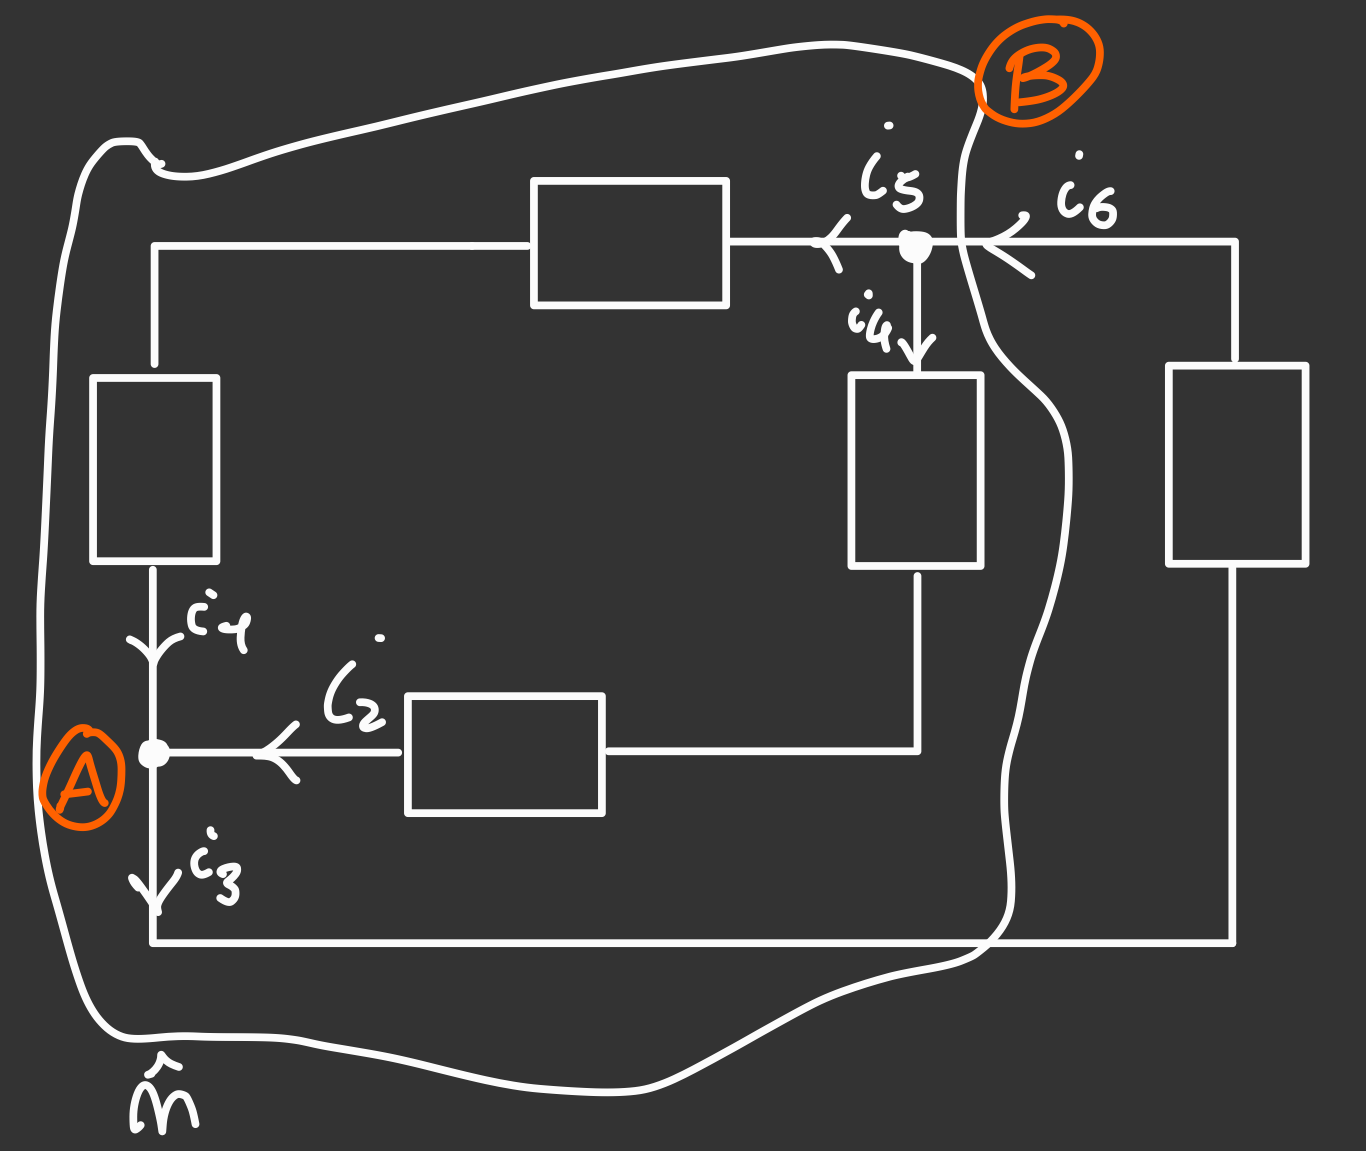
\includegraphics[scale=0.25]{Image/Esempio LKC.png}
\end{center}
Sapendo che il segno di ogni corrente è negativo se entra in un nodo e positivo se ne esce, non è difficile calcolare le correnti nei nodi A e B 
\begin{align*}
    A&: -i_1 -i_2+i_3=0 & B&: -i_5-i_4+i_3=0
\end{align*}


\subsubsection{Teorema di Tellegen}
Combinando la LKT e la LKC su un circuito è possibile verificare che la somma delle potenze dei generatori è pari alla somma delle potenze degli utilizzatori.
\[
    \sum_{k=1}^{n^o \text{ generatori}} p_k = \sum_{j=1}^{n^o \text{ utilizzatori}} p_j
\]










\subsection{Elementi circuitali passivi}
Gli elementi circuitali passivi sono elementi che (nel caso ideale) restituiscono la stessa energia che ricevono. 
\subsubsection{Resistore}
\begin{center}
    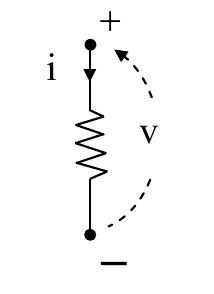
\includegraphics[scale=0.4]{Image/Resistore.png}
\end{center}
\begin{align*}
    &\underbrace{v(t) = R \cdot i(t)}_{1^a\text{ legge di Ohm}} \Longrightarrow i(t) = \dfrac{1}{R} \cdot v(t) & &\underbrace{R = \rho \cdot \dfrac{l}{S}}_{2^a \text{ legge di Ohm}} = \rho \cdot  \dfrac{[\text{lunghezza filo}]}{[\text{sezione filo}]}
\end{align*}
\[
    p(t) = v(t) \cdot i(t) = R \cdot i^2(t) >0
\]
Il resistore assorbe sempre potenza, non può erogarla.


\subsubsection{Condensatore}
\begin{center}
    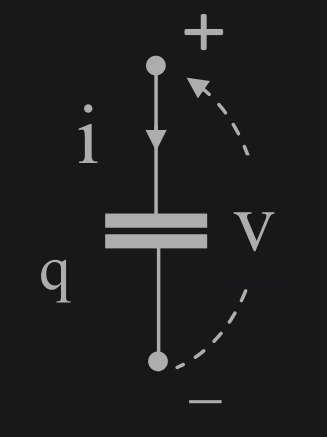
\includegraphics[scale=0.4]{Image/Condensatore.png}
\end{center}
\[
    i = C \cdot \dfrac{dv}{dt} \underset{i=\frac{dq}{dt}}{\Longrightarrow} \frac{dq}{dt} = C \cdot \frac{dv}{dt}
\]
quindi $Q = C \cdot V$.\\
Un condensatore (ideale) è non dissipativo: eroga sempre la stessa quantità di potenza che ha assorbito.
\begin{align*}
    \underbrace{w(t)}_{\text{energia}} &= \int_{t_1}^{t_2} p(t) \ dt\\
    &= \int_{t_1}^{t_2} C v  \frac{dv}{dt} \ dt\\
    &= C \int_{t_1}^{t_2} v \ dv\\
    &= \frac{1}{2} C \left[v^2(t_2) - v^2(t1)\right]
\end{align*}
quindi se consideriamo $t_1=0$ e la tensione $v$ calcolata in un istante finale $t_f$
\[
    w(0,t_f) = \frac{1}{2}Cv^2
\]
$v$ è la variabile di stato del condensatore.
\begin{center}
    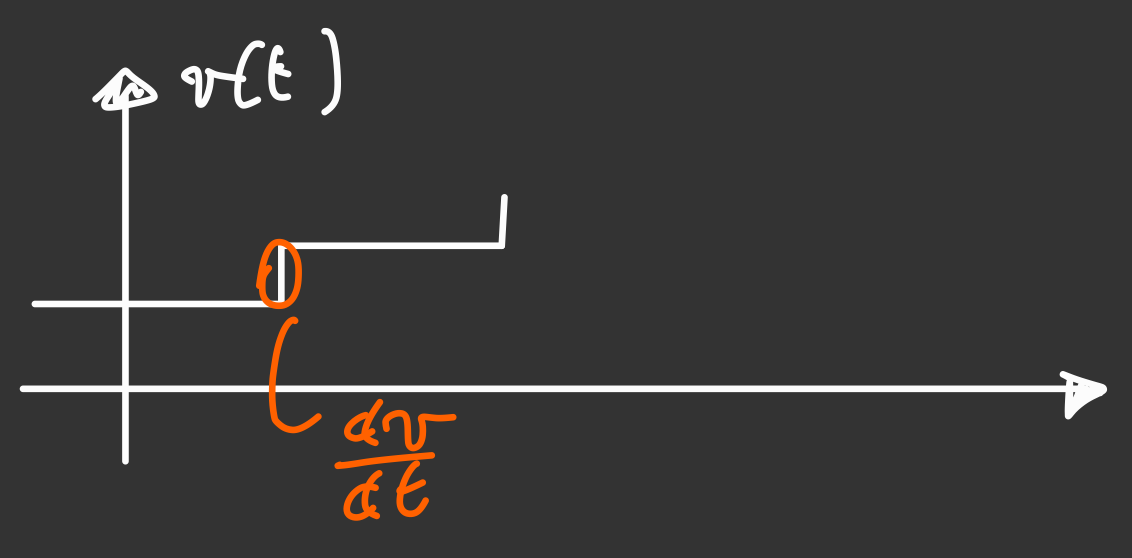
\includegraphics[scale=0.22]{Image/Grafico condensatore.png}
\end{center}
in quel punto $\dfrac{dv}{dt}=\infty \Rightarrow i(t)=\infty \Rightarrow p(t) = \infty$, ma è impossibile avere potenza infinita, quindi non possiamo avere una variazione istantanea di tensione (il grafico della tensione di un condensatore non può avere discontinuità).
\begin{align*}
    i(t) \ dt = C \cdot \frac{dv}{dt} \Longrightarrow \int_{- \infty}^{t} \frac{i(t)}{C} dt = \underbrace{\int_{- \infty}^{t} \frac{dv}{dt}dt}_{v(t)} \Longrightarrow  v(t) &= \int_{- \infty}^{t} \frac{1}{C} \cdot i(t) \ dt\\ 
    &= \underbrace{\int_{- \infty}^{0} \frac{1}{C} \cdot i(t) \ dt}_{v_0} + \int_{0}^{t} \frac{1}{C} \cdot i(t) \ dt
\end{align*}
A differenza del resistore, per conoscere la tensione non ho bisogno solo della corrente nell'istante corrente, ma anche della tensione iniziale; per questo il condensatore è un \textbf{elemento con memoria}.
\vspace*{0.2cm}\\
Un \textbf{condensatore reale} è semplicemente un condensatore messo in parallelo con un resistore.


\subsubsection{Induttore}
L'induttore è un componente elettrico che genera un campo magnetico al passaggio di corrente elettrica.
\begin{center}
    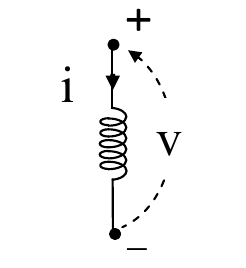
\includegraphics[scale=0.4]{Image/Induttore.png}
\end{center}
\[
    v= L \dfrac{di}{dt}
\]
Sappiamo che la corrente genera un flusso:
\begin{align*}
    &\underbrace{\Phi = L \cdot i}_{I^a\text{ equazione di Maxwell}} & \underbrace{v= \dfrac{d \Phi}{dt}}_{legge di Faraday} = L \dfrac{di}{dt}
\end{align*}
\[
    p(t) = v(t) \cdot i(t) = L \cdot i(t) \dfrac{di}{dt} \begin{cases}
        >0 &\text{assorbita}\\
        <0 &\text{erogata}
    \end{cases}
\]
L'induttore è un elemento \textbf{non dissipativo}.
\begin{align*}
    w(t) &= \int_{t_1}^{t_2} p(t) \ dt\\
    &=L \int_{t_1}^{t_2}i(t) \dfrac{di}{dt} \ dt \\
    &= \dfrac{1}{2} L \left[ i^2(t_2) -i^2(t_1)  \right]
\end{align*}
\[
    w(0,t_f) = \dfrac{1}{2} L \cdot  I^2_f
\]
Anche per l'induttore le variazioni istantanee di tensione non sono possibili.
\begin{center}
    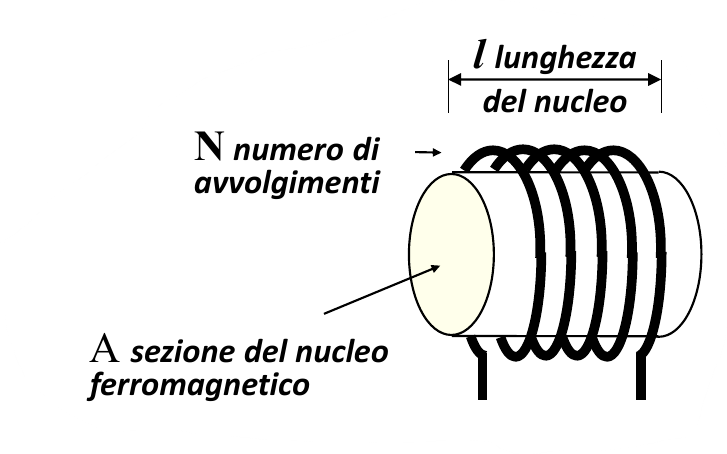
\includegraphics[scale=0.4]{Image/Induttore ferr.png}
\end{center}
\[
   L = \dfrac{\mu  N^2  A}{l} 
\]
\begin{align*}
    i(t) &= \dfrac{1}{L} \int_{- \infty}^{t} v(t) \ dt \\
    &= \dfrac{1}{L} \underbrace{\int_{- \infty}^{0} v(t) \ dt}_{i_0} + \dfrac{1}{L} \int_{0}^{t} v(t) \ dt
\end{align*}
Si vede che anche l'induttore è un elemento \textbf{con memoria}.\\
Un induttore reale è un induttore in serie con un resistore.

\subsubsection{Dispositivi in serie e in parallelo}
\begin{center}
    \begin{tabular}{c c c c}
        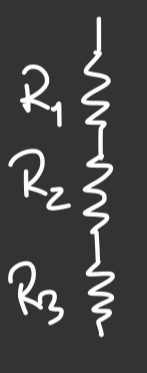
\includegraphics[scale=0.37]{Image/Resistori in serie.png} 
        &
         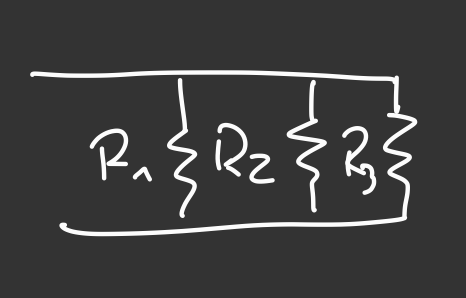
\includegraphics[scale=0.37]{Image/Resistori in parallelo.png} 
        &
        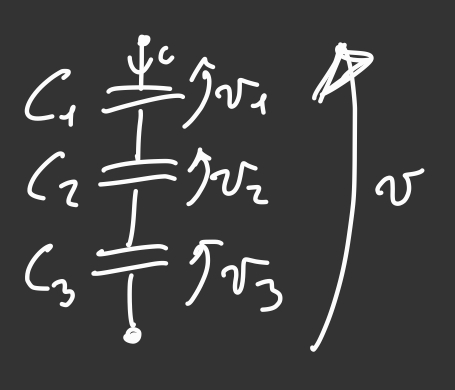
\includegraphics[scale=0.37]{Image/Condensatori in serie.png}
        &
        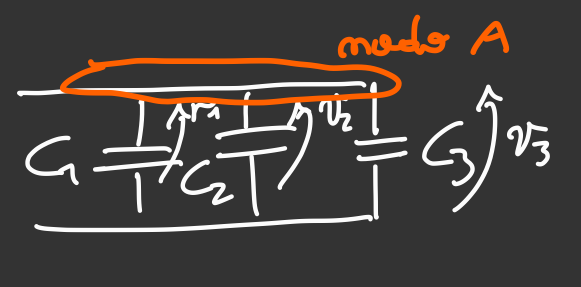
\includegraphics[scale=0.37]{Image/Condensatori in parallelo.png}
        \\
        $R_{eq} = \mathlarger{\sum}_{k=1}^{n}R_k$
        &
        $R_{eq}= \left(\mathlarger{\sum}_{k=1}^n \dfrac{1}{R_k} \right)^{-1} $
        &
        $C_{eq} = \left( \mathlarger{\sum}_{k=1}^{n} \dfrac{1}{C_k} \right)^{-1}$
        &
        $C_{eq} = \mathlarger{\sum}_{k=1}^nC_k$
    \end{tabular}
\end{center}
\begin{center}
    \begin{tabular}{c c}
        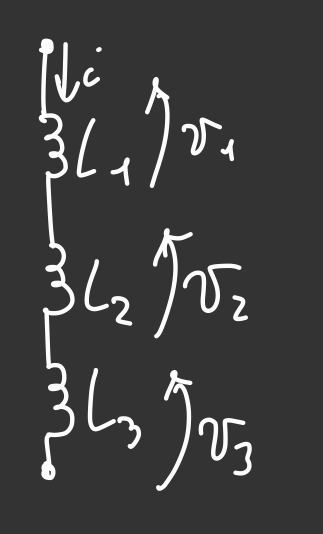
\includegraphics[scale=0.37]{Image/Induttori in serie.png}
        &
        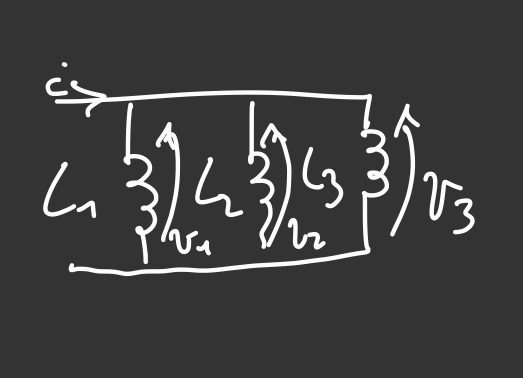
\includegraphics[scale=0.37]{Image/Induttori in parallelo.png}\\
        $L_{eq} = \mathlarger{\sum}_{k=1}^nL_k$
        &
        $ L_{eq} = \left( \mathlarger{\sum}_{k=1}^n \dfrac{1}{L_k} \right)^{-1} $
    \end{tabular}
\end{center}




\subsection{Elementi circuitali attivi}
Gli elementi attivi sono elementi che possono generare (e fornire) energia elettrica.


\subsubsection{Generatore indipendente di tensione}
\begin{center}
    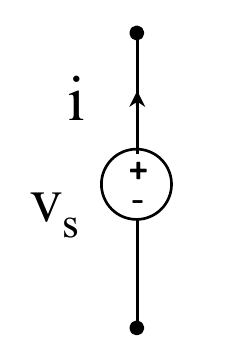
\includegraphics[scale=0.4]{Image/Gen Tensione ideale.png}
\end{center}
Il \textit{generatore di tensione ideale} mantiene
la tensione tra i suoi terminali indipendentemente dalla
corrente che lo attraversa, quindi la tensione ai capi $V$ è uguale alla tensione interna $e$ (N.B. nel disegno la $v_s$ è la tensione interna $e$).
\[
    p(t) = V \cdot i = e \cdot i 
    \begin{cases} 
        >0 &\text{eroga}\\
        <0 &\text{assorbe}\\
    \end{cases}
\]
Essendo $e$ fisso, la potenza dipende solo da $i$ (variabile di stato).
\vspace*{0.2cm}\\
Per simulare un generatore
di tensione reale (ad es. una batteria) si
considera un resistenza
interna $R_i$ in serie con il
generatore ideale:
\begin{center}
    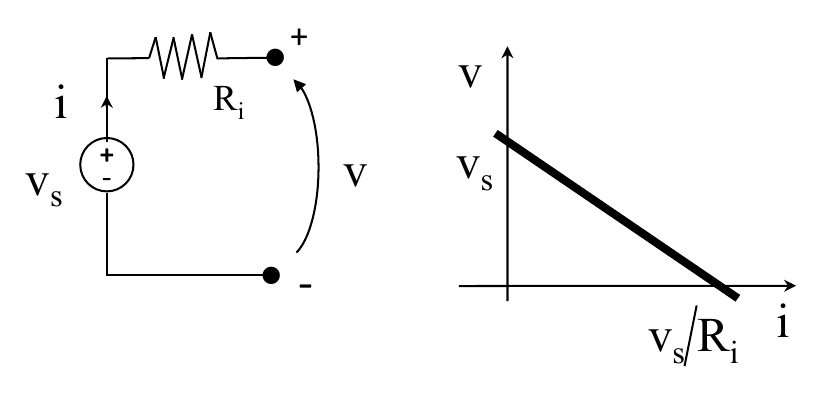
\includegraphics[scale=0.4]{Image/Gen tensione reale.png}
\end{center}
\[
    V = e - R \cdot i
\]
In realtà nella formula della tensione di una batteria ci sono anche termini dipendenti da altri piccoli condensatori nella stessa.
\vspace*{0.2cm}\\
Se si hanno più generatori di tensione \textbf{in serie}, la tensione totale è semplicemente la somma delle tensioni dei vari generatori.\\
I generatori di tensione \textbf{\underline{non sono collegabili in parallelo}}: se così fosse si avrebbero, nella stessa maglia, due differenti tensioni, ma questo non è possibile perché non viene soddisfatta la LKT.
\vspace*{0.2cm}\\
In un generatore di tensione reale, nel caso in cui la resistenza $R \rightarrow \infty \Longrightarrow i = \dfrac{V}{R} = 0$, mentre se $R \rightarrow 0 \Longrightarrow i=\dfrac{V}{R}= \infty$.



\subsubsection{Generatore indipendente di corrente}
\begin{center}
    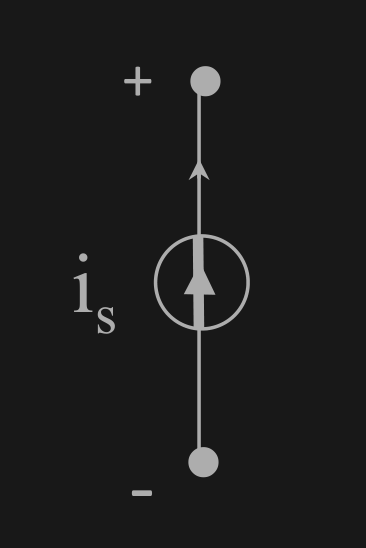
\includegraphics[scale=0.4]{Image/Gen corrente ideale.png}
\end{center}
Il \textit{generatore di corrente ideale} mantiene
la corrente che lo attraversa al valore $ A $ indipendentemente dalla
differenza di potenziale fra i suoi terminali (N.B. nel disegno la $i_s$ è la corrente interna $A$).
\[
    p(t) = V \cdot i = V \cdot A 
    \begin{cases}
        >0 &\text{eroga}\\
        <0 &\text{assorbe}
    \end{cases}
\]
Un imprecisa approssimazione di un generatore di corrente reale è un pannello fotovoltaico, dotato di resistenza interna in parallelo con il generatore ideale
\begin{center}
    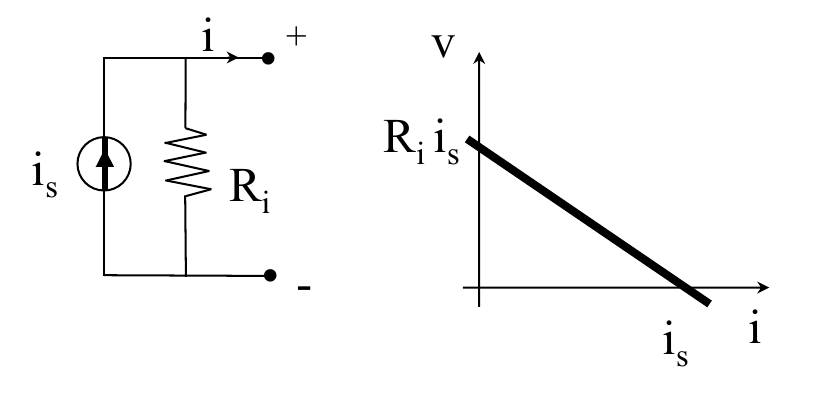
\includegraphics[scale=0.4]{Image/Gen corrente reale.png}
\end{center}
\[
    i = A -\frac{v}{R}
\]


\subsubsection{Generatori dipendenti}
Gli elementi attivi visti prima possono essere "controllati" in tensione o in corrente.
\vspace*{0.2cm}\\
Il \textbf{generatore dipendente di tensione} è controllato in tensione $V=v_c \cdot  \mu$, o in corrente $V = r \cdot i_c$.
\vspace*{0.2cm}\\
Il \textbf{generatore dipendente di corrente} è controllato in tensione $i = g \cdot v_c$, o in corrente $i = \alpha \cdot i_c$.



\subsection{Circuiti nel dettaglio}
\subsubsection{Circuiti aperti e chiusi}
Un ramo in circuito aperto si può
considerare nei due seguenti modi:
\begin{itemize}
    \item Un generatore di corrente con: $A = 0$
    \item Un resistore con: $R = + \infty$
\end{itemize}
L'equazione dell'elemento circuitale è $i=0, \ \forall v$.
\begin{center}
    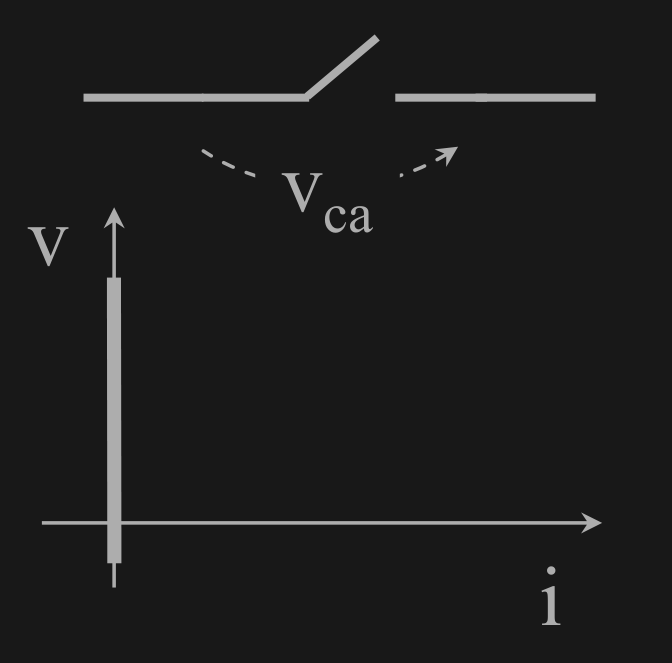
\includegraphics[scale=0.35]{Image/Circuito aperto.png}
\end{center}
Un ramo in circuito chiuso si può
considerare nei due seguenti modi:
\begin{itemize}
    \item Un generatore di tensione con: $e = 0$
    \item Un resistore con: $R = 0$
\end{itemize}
L'equazione dell'elemento circuitale è $v=0, \ \forall i$.
\begin{center}
    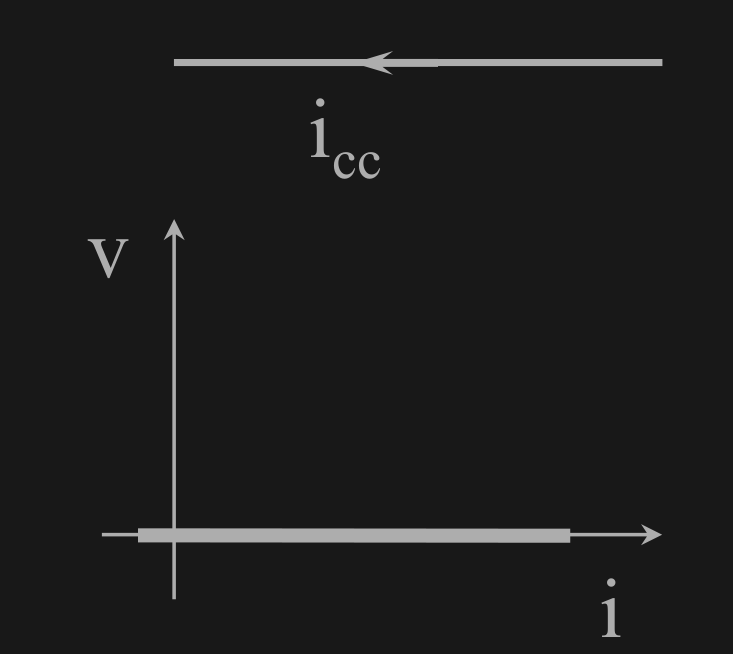
\includegraphics[scale=0.35]{Image/Circuito chiuso.png}
\end{center}
\begin{center}
    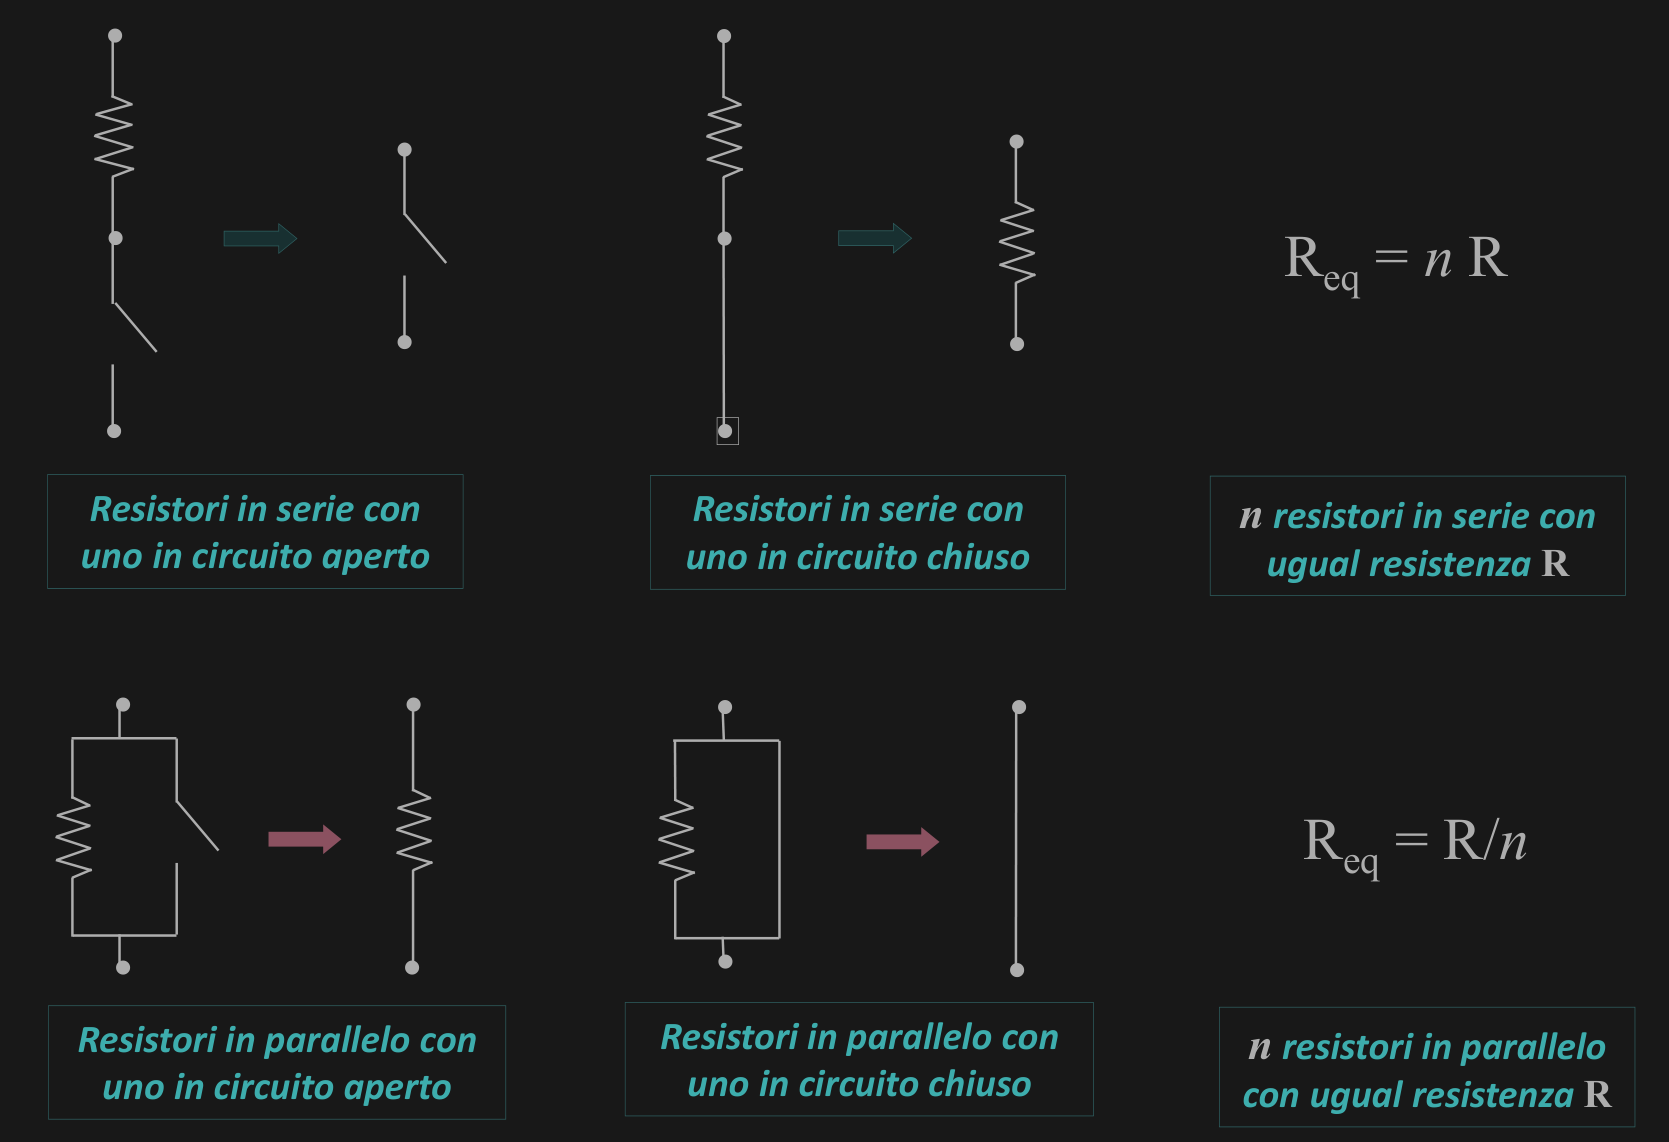
\includegraphics[scale=0.3]{Image/Resistori aperto chiuso.png}
\end{center}


\subsubsection{Esempio 1}
\begin{center}
    \begin{tabular}{c c c c}
    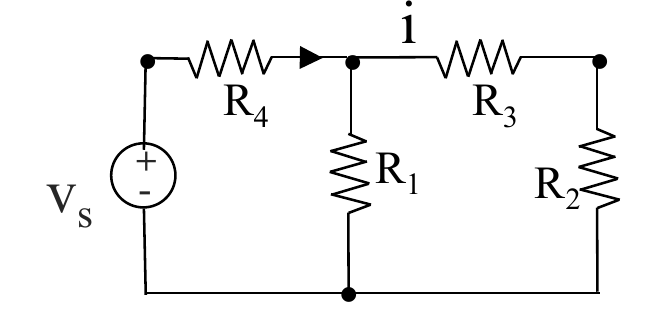
\includegraphics[scale=0.25]{Image/Esempio1_1.png}
    &
    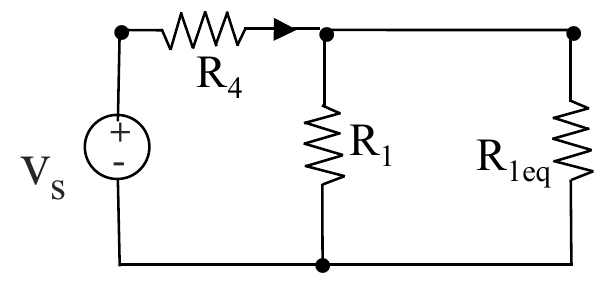
\includegraphics[scale=0.25]{Image/Esempio1_2.png}
    &
    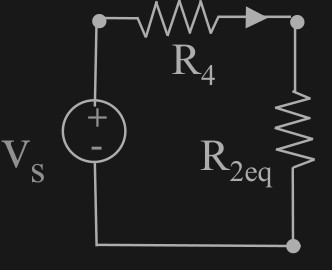
\includegraphics[scale=0.27]{Image/Esempio1_3.png}
    & 
    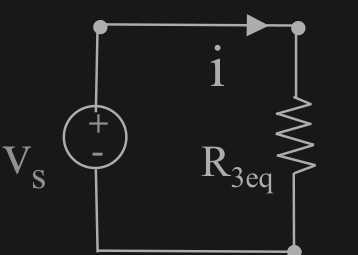
\includegraphics[scale=0.27]{Image/Esempio1_4.png}\\
    &
    $R_{1eq} = R_2+R_3$
    &
    $R_{2eq} =\dfrac{R_1 R_{1eq}}{R_1+R_{1eq}} = \left( \dfrac{1}{R_1} + \dfrac{1}{R_{1eq}} \right)^{-1}$
    &
    $R_{3eq} = R_4 + R_{2eq} $
\end{tabular}
\end{center}


\subsubsection{Partitore di tensione}
Un partitore di tensione è un tipo di circuito costituito da due o più componenti passivi collegati in serie ai capi dei quali, se viene applicata una tensione, essa si ripartirà sulle stesse componenti in base al loro valore. La legge generale si ottiene moltiplicando il valore della tensione applicata alla serie per il rapporto tra la resistenza ai capi della quale si vuole conoscere la tensione e la somma delle resistenze componenti la serie.
\begin{center}
    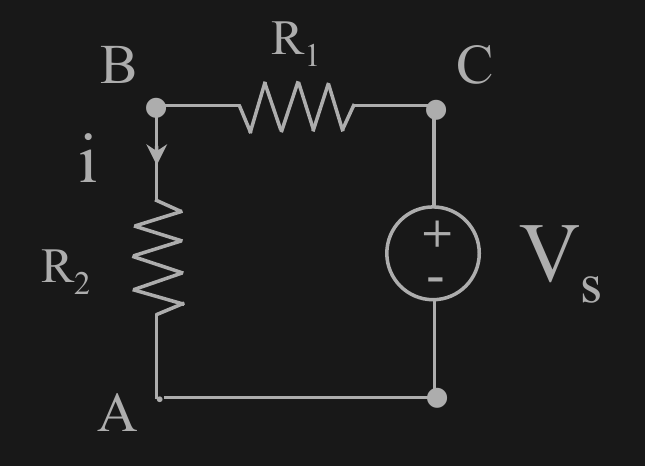
\includegraphics[scale=0.35]{Image/Partitore di tensione.png}
\end{center}
\begin{align*}
    R_{eq} &= R_1+R_2 & i = \dfrac{V_s}{R_{eq}} = \dfrac{V_s}{R_1+R_2}
\end{align*}
Dalla LKT si ha
\begin{align*}
    &v_1+v_2 - V_s = 0 \Longrightarrow & v_1&=V_s - v_2 = V_s - R_2 i & v_2 &= V_s-v_1 = V_s - R_1 i\\
    &\underset{\text{sostituisco } i}{\Longrightarrow} & v_1&=\dfrac{R_1}{R_1+R_2} V_s & v_2&=\dfrac{R_2}{R_1+R_2} V_s
\end{align*}


\subsubsection{Partitore di corrente}
Il partitore di corrente è un circuito utilizzato per ottenere la corrente elettrica che scorre attraverso un'impedenza o attraverso un circuito quando esso viene connesso in parallelo con un'altra impedenza. La differenza sostanziale con il partitore di tensione è che in questo caso, nella formula, al numeratore della frazione va la resistenza che non si sta considerando.
\begin{center}
    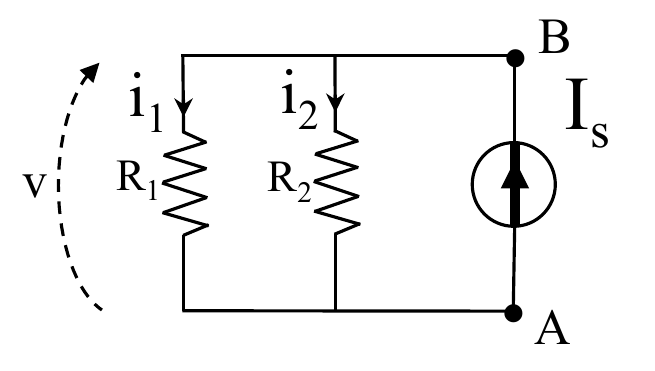
\includegraphics[scale=0.35]{Image/Partitore di corrente.png}
\end{center}
\begin{align*}
    R_{eq} &= \dfrac{R_1R_2}{R_1+R_2} & v &= R_{eq}I_s = \dfrac{R_1R_2}{R_1+R_2}I_s
\end{align*}
Dalla LKC si ha
\begin{align*}
    &i_1 + i_2 -I_s = 0 \Longrightarrow & i_1 &= I_s - i_2 = I_s - \dfrac{v}{R_2} &  i_2 &= I_s - i_1 = I_s - \dfrac{v}{R_1}\\
    &\underset{\text{sostituisco } v}{\Longrightarrow} & i_1 &= \dfrac{R_2}{R_1+R_2}I_s &  i_2 &= \dfrac{R_1}{R_1+R_2}I_s
\end{align*}






\subsubsection{Collegamenti di resistori a stella e a triangolo}
Un sistema di tre resistenze
può essere collegato a
triangolo o a stella. Può essere
meglio per l'analisi circuitale
una connessione a stella invece
che un triangolo o viceversa.
Da sottolineare che \underline{una rete a stella può essere equivalente ad una rete a} \underline{triangolo}.
\begin{center}
    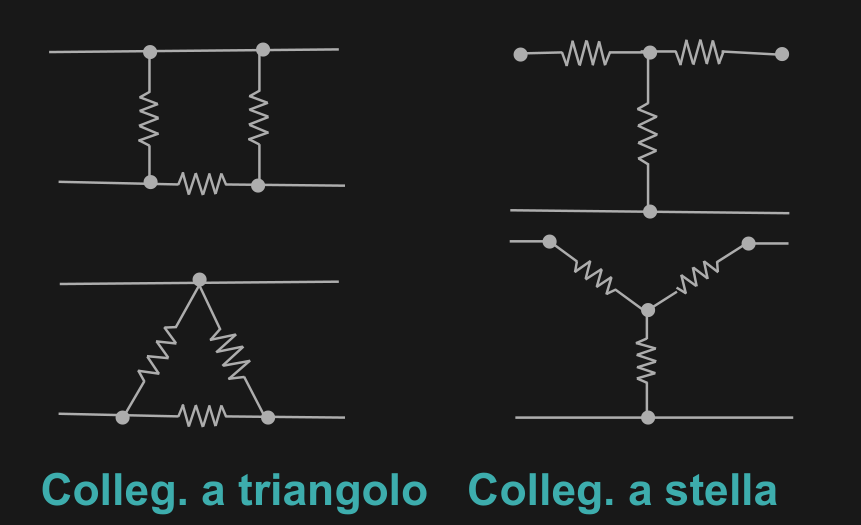
\includegraphics[scale=0.3]{Image/Stella triangolo.png}
    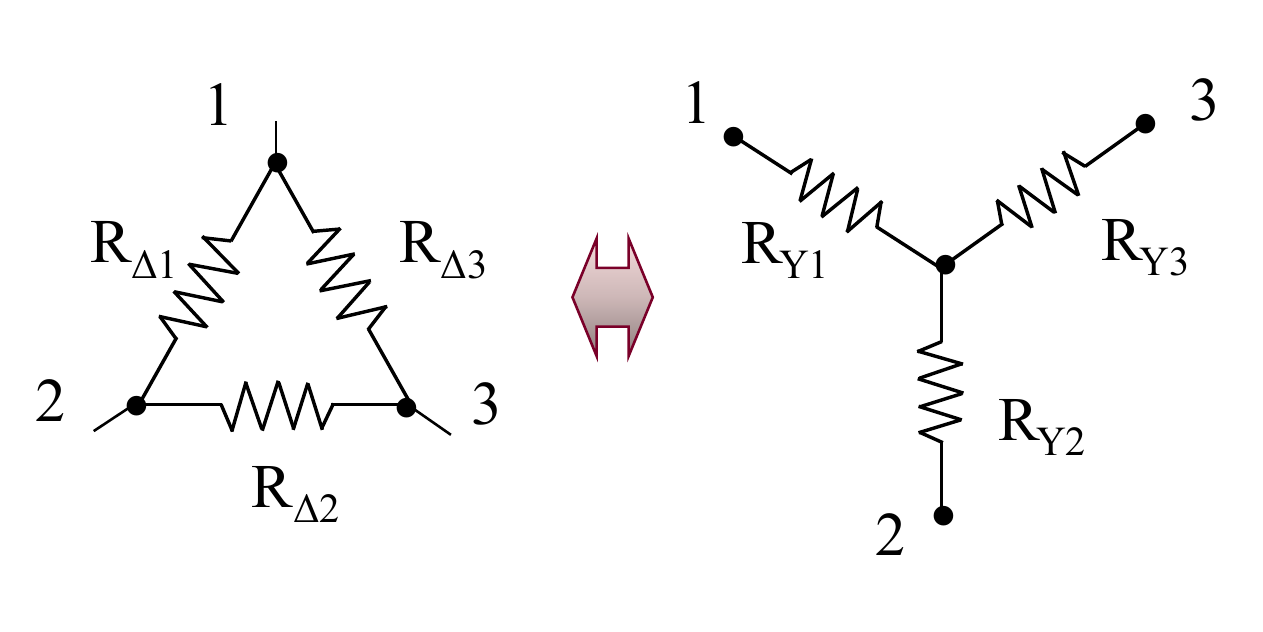
\includegraphics[scale=0.3]{Image/Nodi triangolo stella.png}
\end{center}
Ciò significa che le stesse tensioni $v_{12}$, $v_{23}$ e $v_{31}$ tra i nodi 1 e
2, i nodi 2 e 3 e i nodi 3 e 1 inducono le
stesse correnti entranti nella
stella e nel triangolo rispettivamente al nodo 1,
al nodo 2 ed al nodo 3.
Ora vediamo come passare da stella a triangolo e viceversa
\begin{center}
    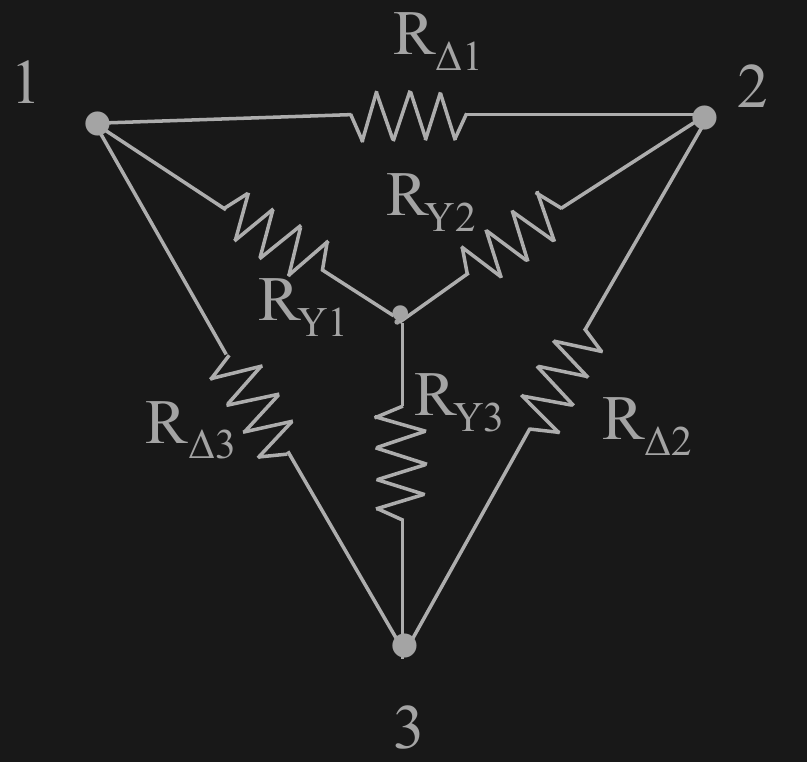
\includegraphics[scale=0.23]{Image/Stella triangolo insieme.png}
\end{center}
Ogni resistenza della stella è il prodotto dei due
resistori del triangolo collegati allo stesso nodo,
diviso per la somma dei resistori a triangolo.
\begin{align*}
    R_{Y1} &= \dfrac{R_{\Delta 1} R_{\Delta 3}}{R_{\Delta 1} + R_{\Delta 2} + R_{\Delta 3}} &
    R_{Y2} &= \dfrac{R_{\Delta 1} R_{\Delta 2}}{R_{\Delta 1} + R_{\Delta 2} + R_{\Delta 3}} &
    R_{Y3} &= \dfrac{R_{\Delta 2} R_{\Delta 3}}{R_{\Delta 1} + R_{\Delta 2} + R_{\Delta 3}}
\end{align*}
Ogni resistenza del triangolo è la somma dei prodotti a due a due di tutti i
resistori della stella, divisa per la resistenza nel ramo opposto della stella.
\begin{align*}
    R_{\Delta 1} &= \dfrac{R_{Y_1}R_{Y_2} +R_{Y2}R_{Y3} + R_{Y3}R_{Y1}}{R_{Y_3}} &
    R_{\Delta 2} &= \dfrac{R_{Y_1}R_{Y_2} +R_{Y2}R_{Y3} + R_{Y3}R_{Y1}}{R_{Y_1}} &
    R_{\Delta 1} &= \dfrac{R_{Y_1}R_{Y_2} +R_{Y2}R_{Y3} + R_{Y3}R_{Y1}}{R_{Y_2}}
\end{align*}
Per $R_{Y1} = R_{Y2} = R_{Y3} = R_Y$ risulta $R_{\Delta 1} = R_{\Delta 2} = R_{\Delta 3} = R_{\Delta}$ e viceversa:
\begin{align*}
    &R_Y = R_{\Delta}/3
    &
    &R_{\Delta} = 3R_Y
\end{align*}





\subsubsection*{Esempio 2}
Determinare la resistenza equivalente del seguente circuito
\begin{center}
    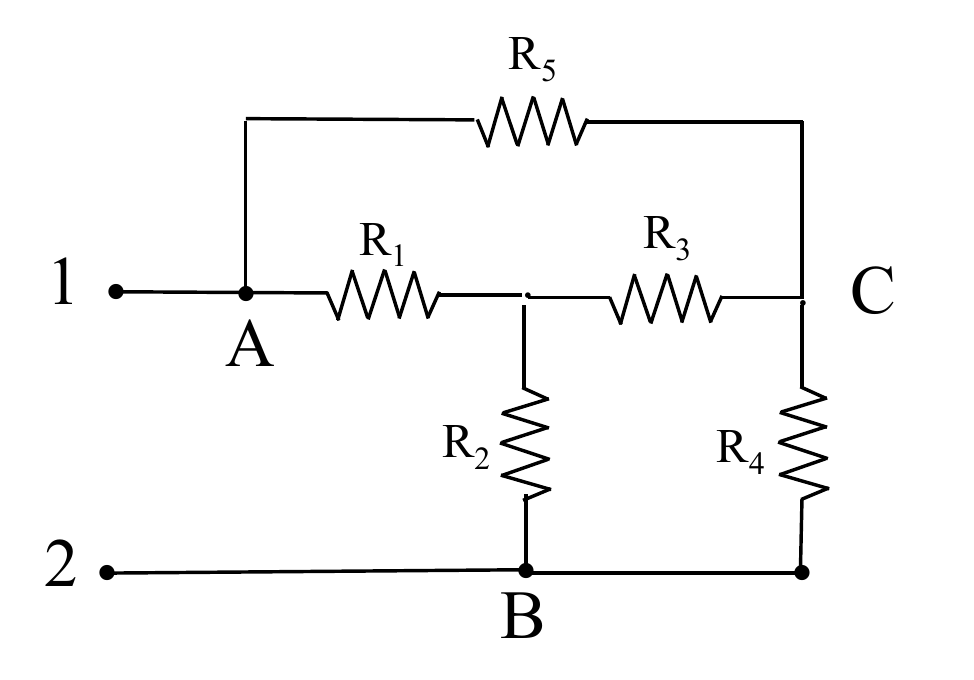
\includegraphics[scale=0.3]{Image/Esempio2_1.png}
\end{center}
\begin{align*}
    R_1&=3 \Omega & R_2&=3 \Omega & R_3&=3 \Omega\\
    R_4&=2 \Omega & R_5&=2 \Omega
\end{align*}
\begin{center}
    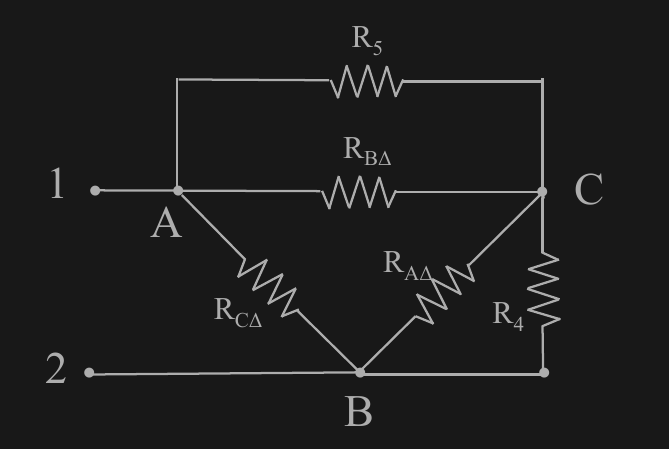
\includegraphics[scale=0.3]{Image/Esempio2_2.png}
\end{center}
\begin{align*}
    R_{A\Delta} &= \dfrac{R_1R_2 + R_2R_3 +R_1R_3}{R_1} = 9 \Omega
    &
    R_{B\Delta} &= \dfrac{R_1R_2 + R_2R_3 +R_1R_3}{R_2} = 9 \Omega
    &
    R_{c\Delta} &= \dfrac{R_1R_2 + R_2R_3 +R_1R_3}{R_3} = 9 \Omega
\end{align*}
\begin{center}
    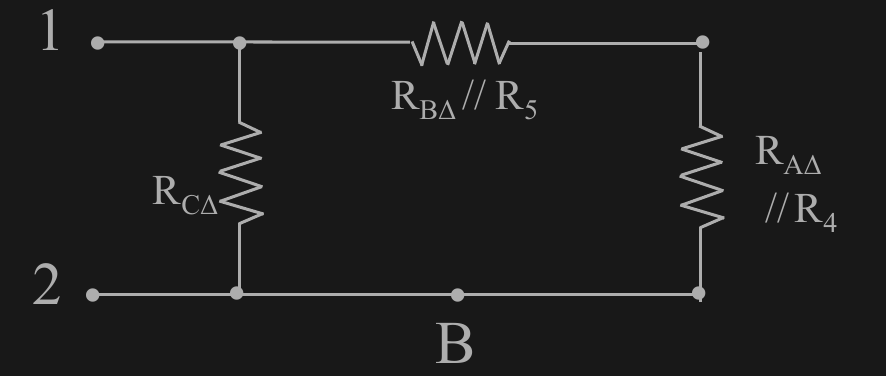
\includegraphics[scale=0.3]{Image/Esempio2_3.png}
\end{center}
\begin{align*}
    R_{B\Delta // R_5} &= \dfrac{R_{B\Delta R_5}}{R_{B\Delta} + R_5} = 1,6364 \Omega & R_{A\Delta // R_4} &= \dfrac{R_{A\Delta R_4}}{R_{A\Delta} + R_4} = 1,6364 \Omega
\end{align*}
\begin{center}
    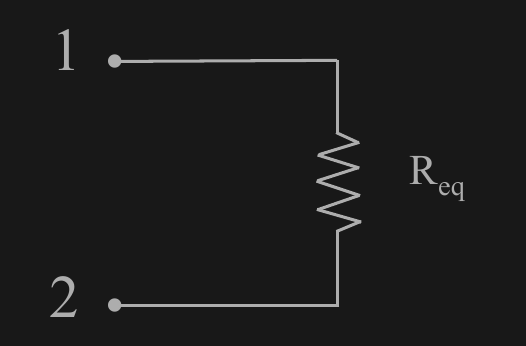
\includegraphics[scale=0.3]{Image/Esempio2_4.png}
\end{center}
\[
    R_{eq} = R_{C\Delta} // (R_{B\Delta} // R5 + R_{A\Delta} // R4) = (9)//(3,272) = 2,41 \Omega
\]







\section{Metodi di analisi}
\subsection{Metodo di Tanenblau}
Prendiamo un circuito di riferimento
\begin{center}
    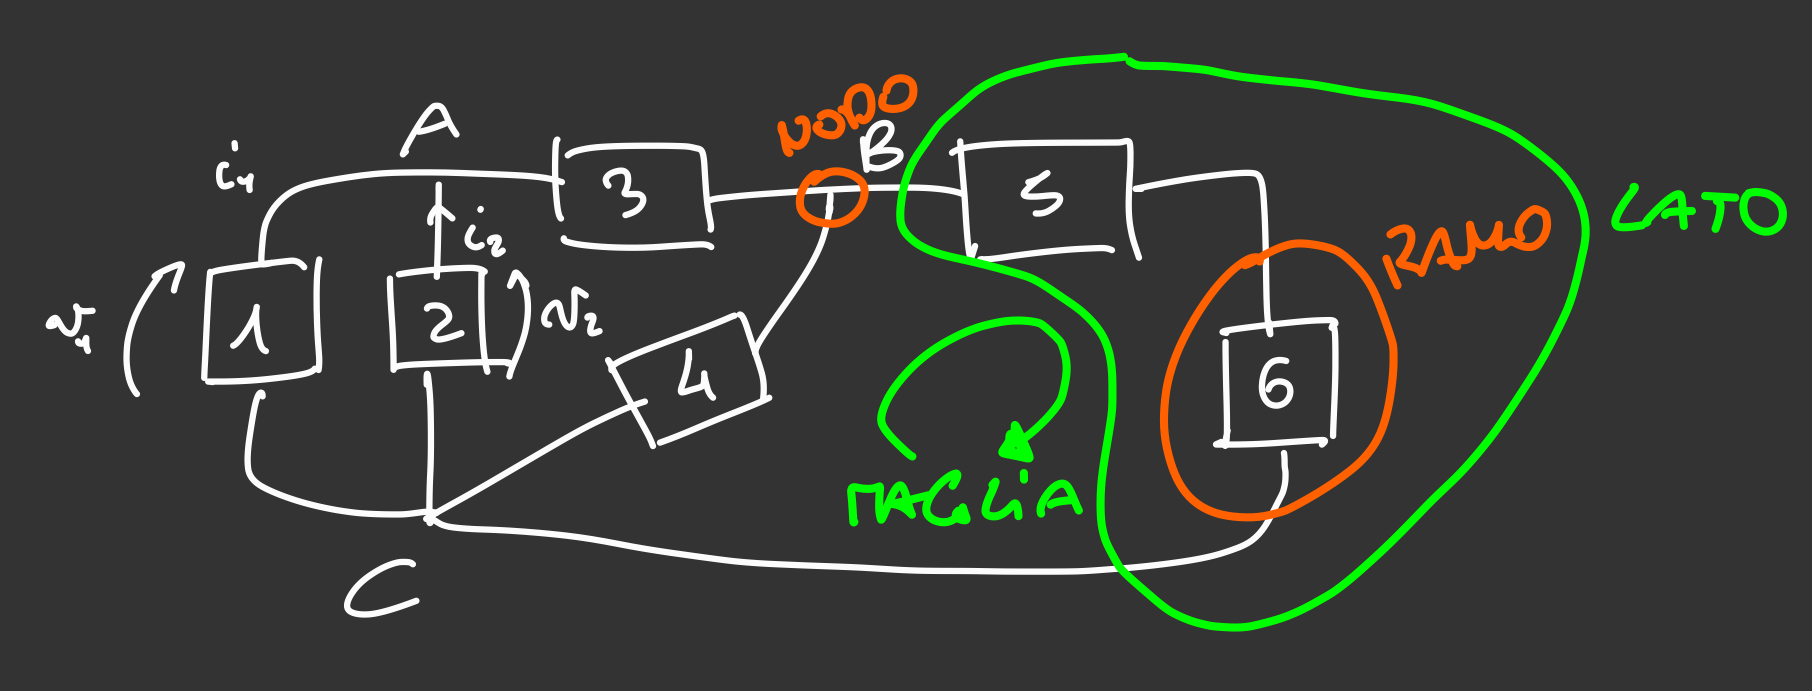
\includegraphics[scale=0.35]{Image/Metodo di Tanenblau_1.png}
\end{center}
Definiamo
\begin{itemize} 
    \item Nodo: intersezione tra 3 o più fili
    \item Ramo: Parte di circuito compresa tra due nodi
    \item Maglia: qualsiasi percorso chiuso del circuito
    \item Lato: connessione in successione di più rami
\end{itemize}
Possiamo riformulare la definizione di risoluzione di un circuito: calcolare tutte le tensioni di lato e tutte le correnti di lato.\\
Quindi se $L$ è il numero di lati, avremo $L$ tensioni e $L$ correnti in un circuito; in totale si hanno $2L$ incognite, che necessitano di $2L$ equazioni indipendenti.
\vspace*{0.2cm}\\
Possiamo scrivere $L$ equazioni costitutive dei componenti, le altre $L$ equazioni di ricavano da LKC e LKT.
\begin{center}
    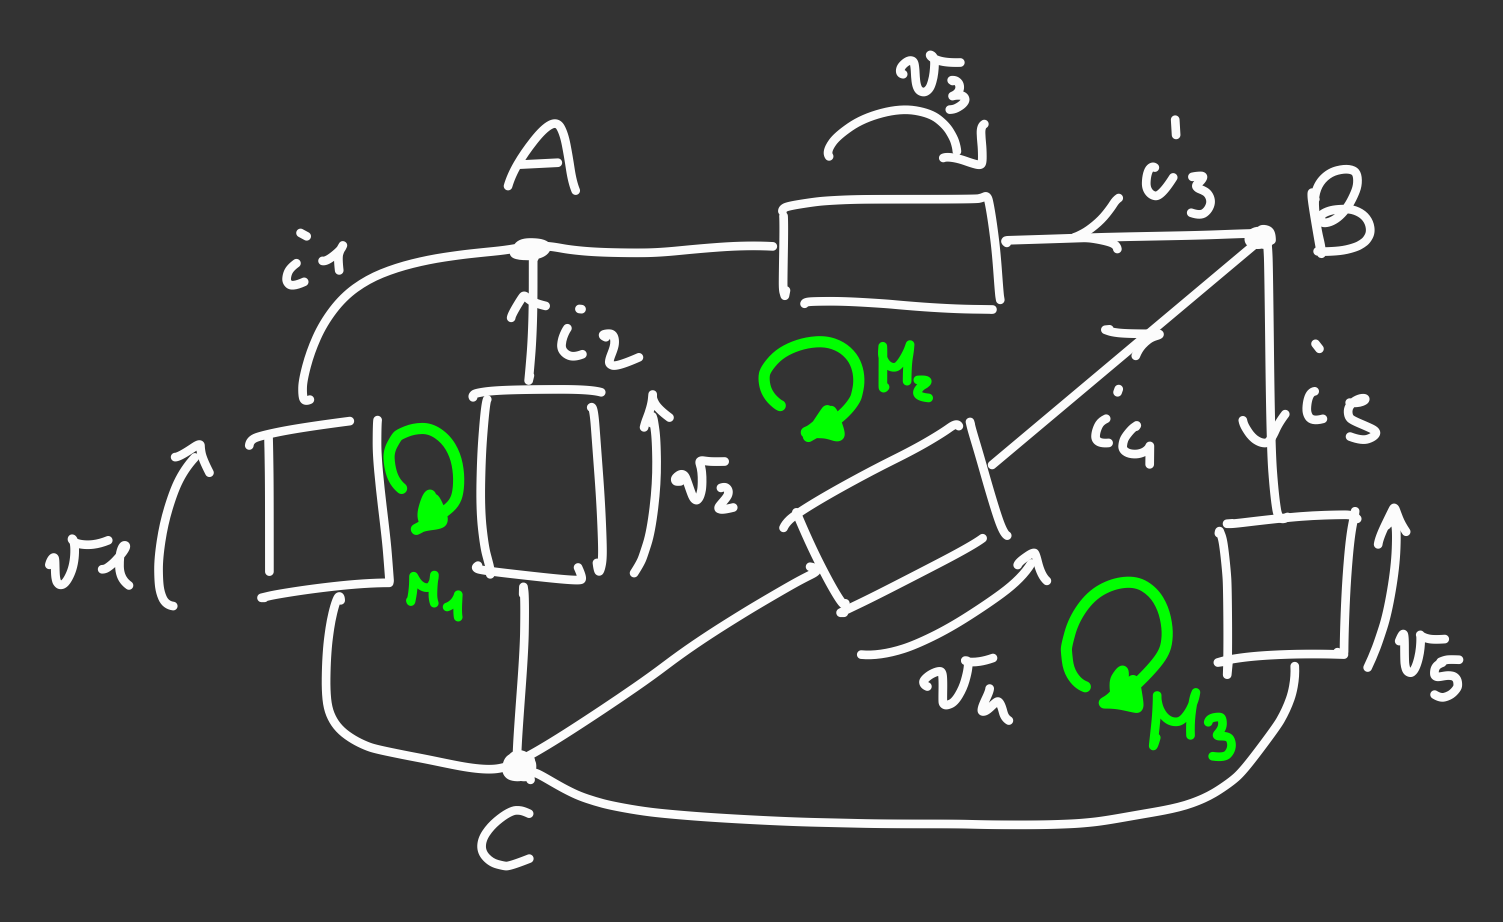
\includegraphics[scale=0.3]{Image/Metodo di Tanenblau_2.png}
\end{center}
\begin{align*}
    &\begin{rcases}
        A(LKC): i_1+i_3-i_2=0\\
        B(LKC): i_4-i_3-i_5=0
    \end{rcases}+ = -i_2 =i_5+i_1+i_4\\
    &C(LKC): i_2+i_5-i_1-i_4=0
\end{align*}
La somma delle prime due equazioni è uguale alle terza con segni invertiti, quindi le tre equazioni non sono indipendenti, solo due di esse lo sono.
\vspace*{0.1cm}\\
Le equazioni che servono per risolvere un circuito sono:
\begin{itemize}
    \item $L$ equazioni costitutive
    \item $N-1$ LKC
    \item $L-N+1$ LKT (maglie non intersecate da rami)
\end{itemize}
Infatti per il circuito avremo
\begin{align*}
    &M_1: v_1-v_2 = 0 & M_3: v_2+v_3 - v_4=0\\
    &M_2: v_4-v_5=0
\end{align*}

\subsubsection*{Passaggi}
\begin{enumerate}
    \item individuare $N$ nodi e $L$ lati
    \item individuare $2L$ incognite ($v,i$)
    \item scrivere le $L$ equazioni di lato
    \item scrivere le $N-1$ LKC e $L-N+1$ LKT
    \item Risolvere il sistema di equazioni
\end{enumerate}

\subsubsection{Esempio}
\begin{center}
    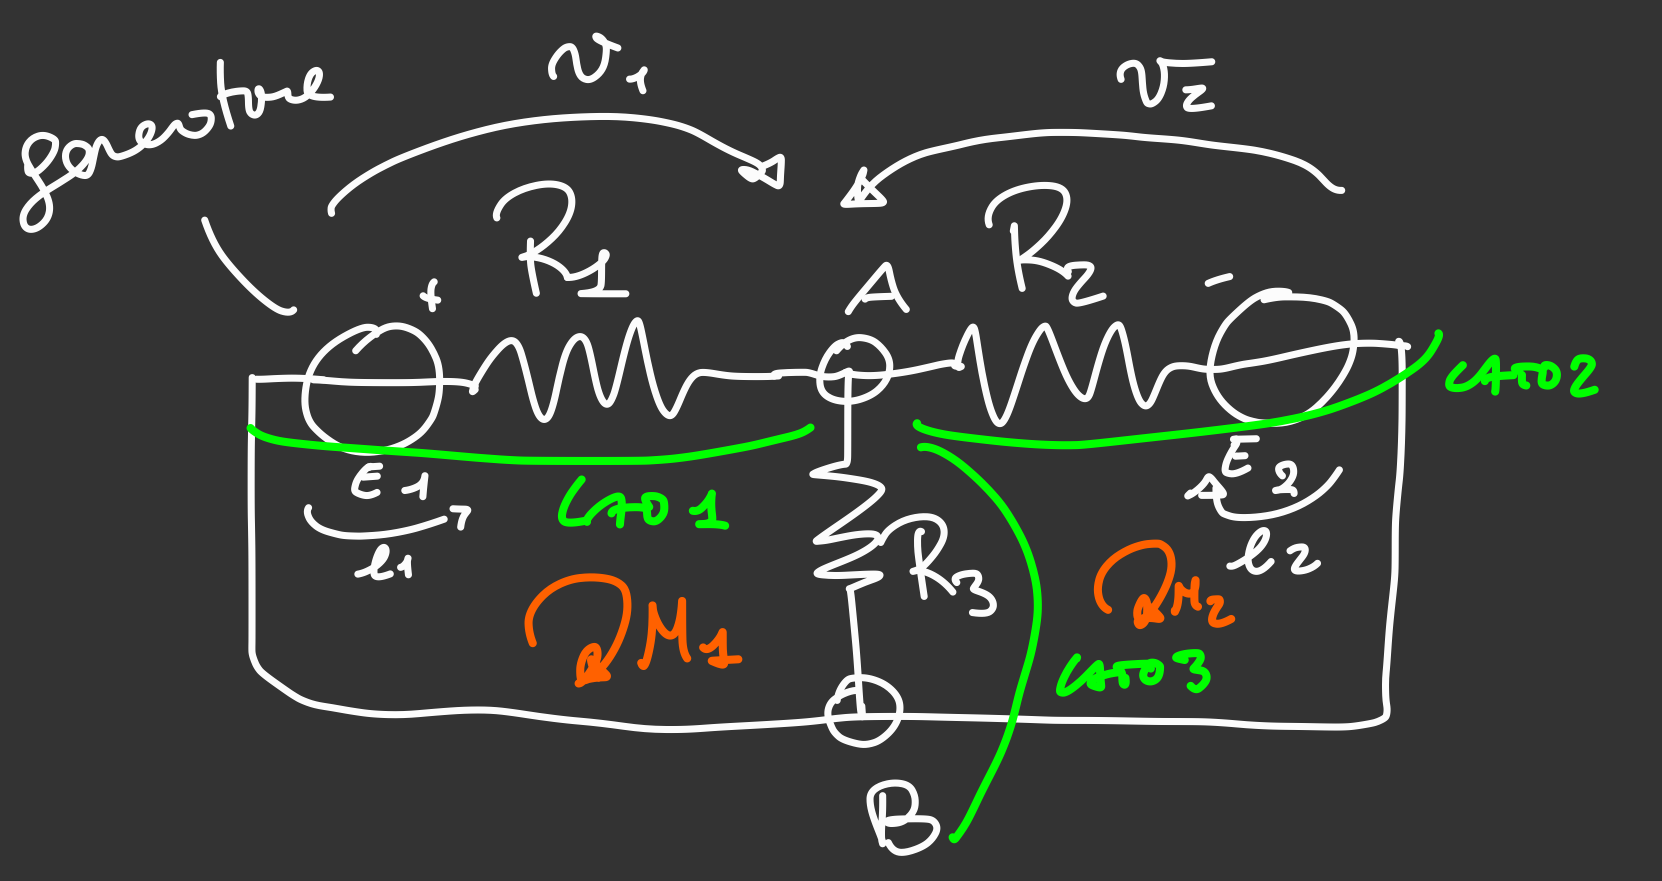
\includegraphics[scale=0.3]{Image/Esempio_Tanenblau.png}
\end{center}

\begin{center}
\begin{tabular}{c|c}
    Equazioni di lato & Equazioni topologiche\\
    \hline
    Lato 1:
    $
    \begin{rcases}
        e_1=E_1\\
        v_{R_1} = R_1 \cdot i_1 
    \end{rcases}
    v_1 = E_1 - R_1 \cdot i_i$
    &
    LKC(A): $i_1+i_2-i_3=0$\\
    Lato 2: 
    $
    \begin{rcases}
        e_2 = E_2\\
        v_{R_2} = R_2 \cdot i_2
    \end{rcases}
    v_2 = E_2 - R_2 \cdot i_2
    $
    &
    LKT($M_1$) : $v_1 - v_3=0$\\
    Lato 3: $v_{R_3} = R_3 \cdot i_3$ 
    &
    LKT($M_2$) : $v_3-v_2=0$    
\end{tabular}
\end{center}
Ora effettuiamo la sostituzione:
\[
    \begin{rcases}
        v_1 - v_3 = E_1-R_1i_1 - R_3i_3=0\\
        v_3 - v_2 = R_3i_3 - E_2 + R_2i_2=0
    \end{rcases}
    \Longrightarrow
    \begin{cases}
        i_1+i_2-i_3=0\\
        R_1i_1+R_3i_3=E_1\\
        R_2i_2+R_3i_3=E_2
    \end{cases}
\]







\subsection{Metodo dei potenziali di nodo}
\begin{enumerate}
    \item scegliere un nodo di rifermento
    \item assegniamo le tensioni agli altri nodi
    \item LKC ai nodi non di riferimento
    \item scrivere le correnti in funzione dei potenziali di nodo
    \item risolvere infine il sistema di equazioni
\end{enumerate}



\subsection{Esempio}
\begin{center}
    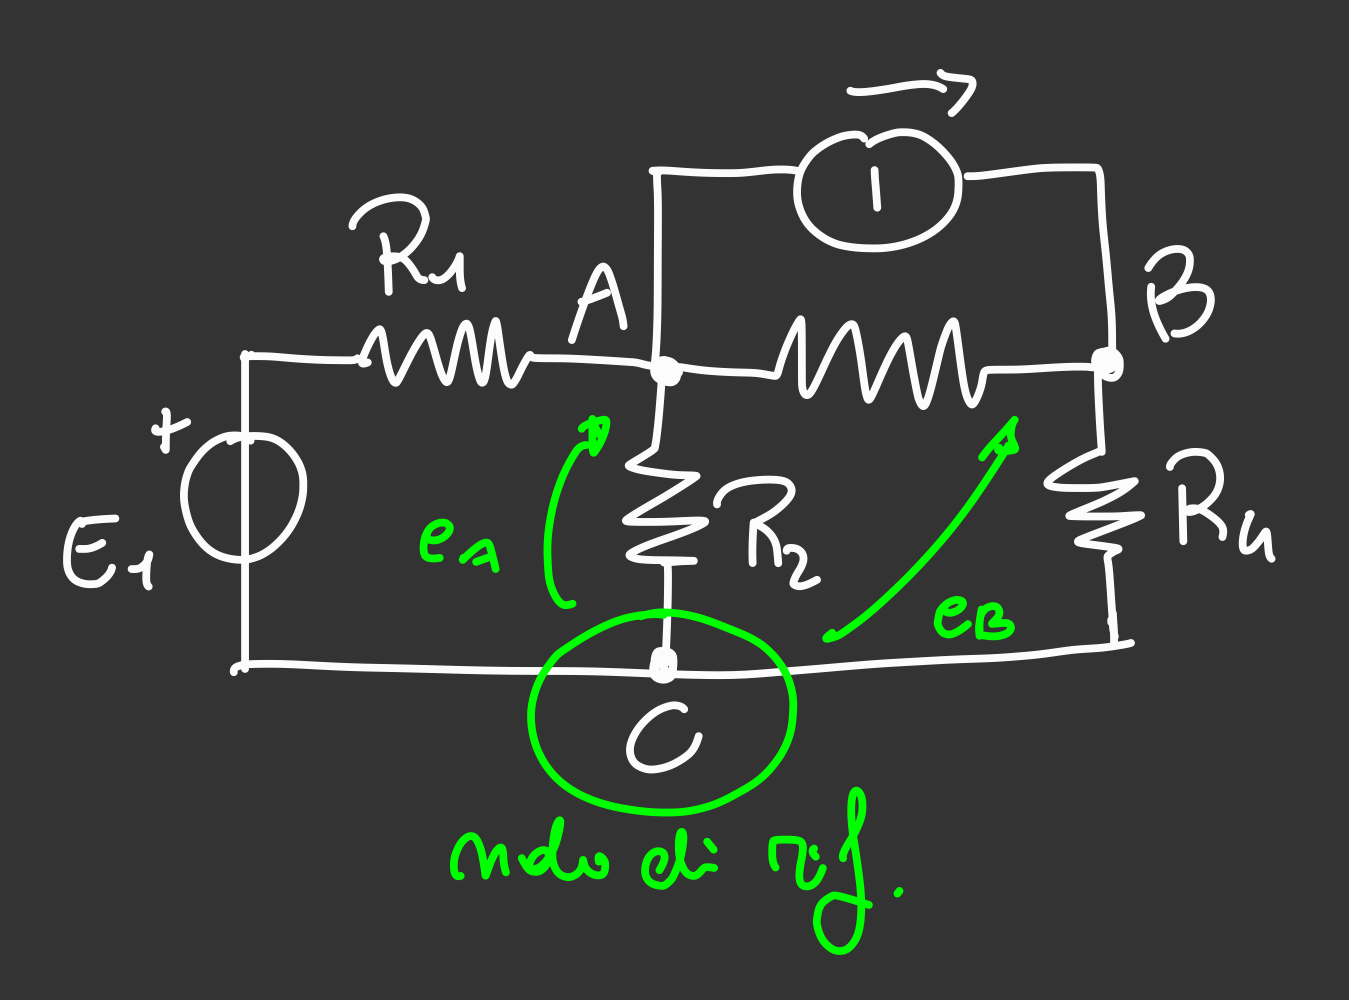
\includegraphics[scale=0.12]{Image/Esempio_PotenzialiNodo.png}
\end{center}
Scegliamo come nodo di riferimento il nodo C
\begin{align*}
    \text{LKC(A): }&i_1-i_2 - I - i_3=0\\
    \text{LKC(B): }&i_3 + I - i_4=0\\
\end{align*}
\begin{align*}
    &i_1=\dfrac{E_1-e_A}{R_1} & &i_2 = \dfrac{e_A}{R_2} & &i_3 = \dfrac{e_A-e_B}{R_3}
\end{align*}







\subsection{Teoremi di rete}
\subsubsection*{Ipotesi di linearità}
 $f(x_1+x_2)$ è lineare
\begin{align*}
    \text{additività: } &f(x_1+x_2) = f(x_1) + f(x_2)\\
    \text{omogeneità: } &f(ax_1) = af(x_1)
\end{align*}

\subsection{Sovrapposizione degli effetti}
Ipotesi: circuito lineare.\\
Le variabili di rete (effetti) si possono ottenere come sovrapposizione delle risposte dovute alle singole cause.

\subsubsection{Esempio}
\begin{center}
    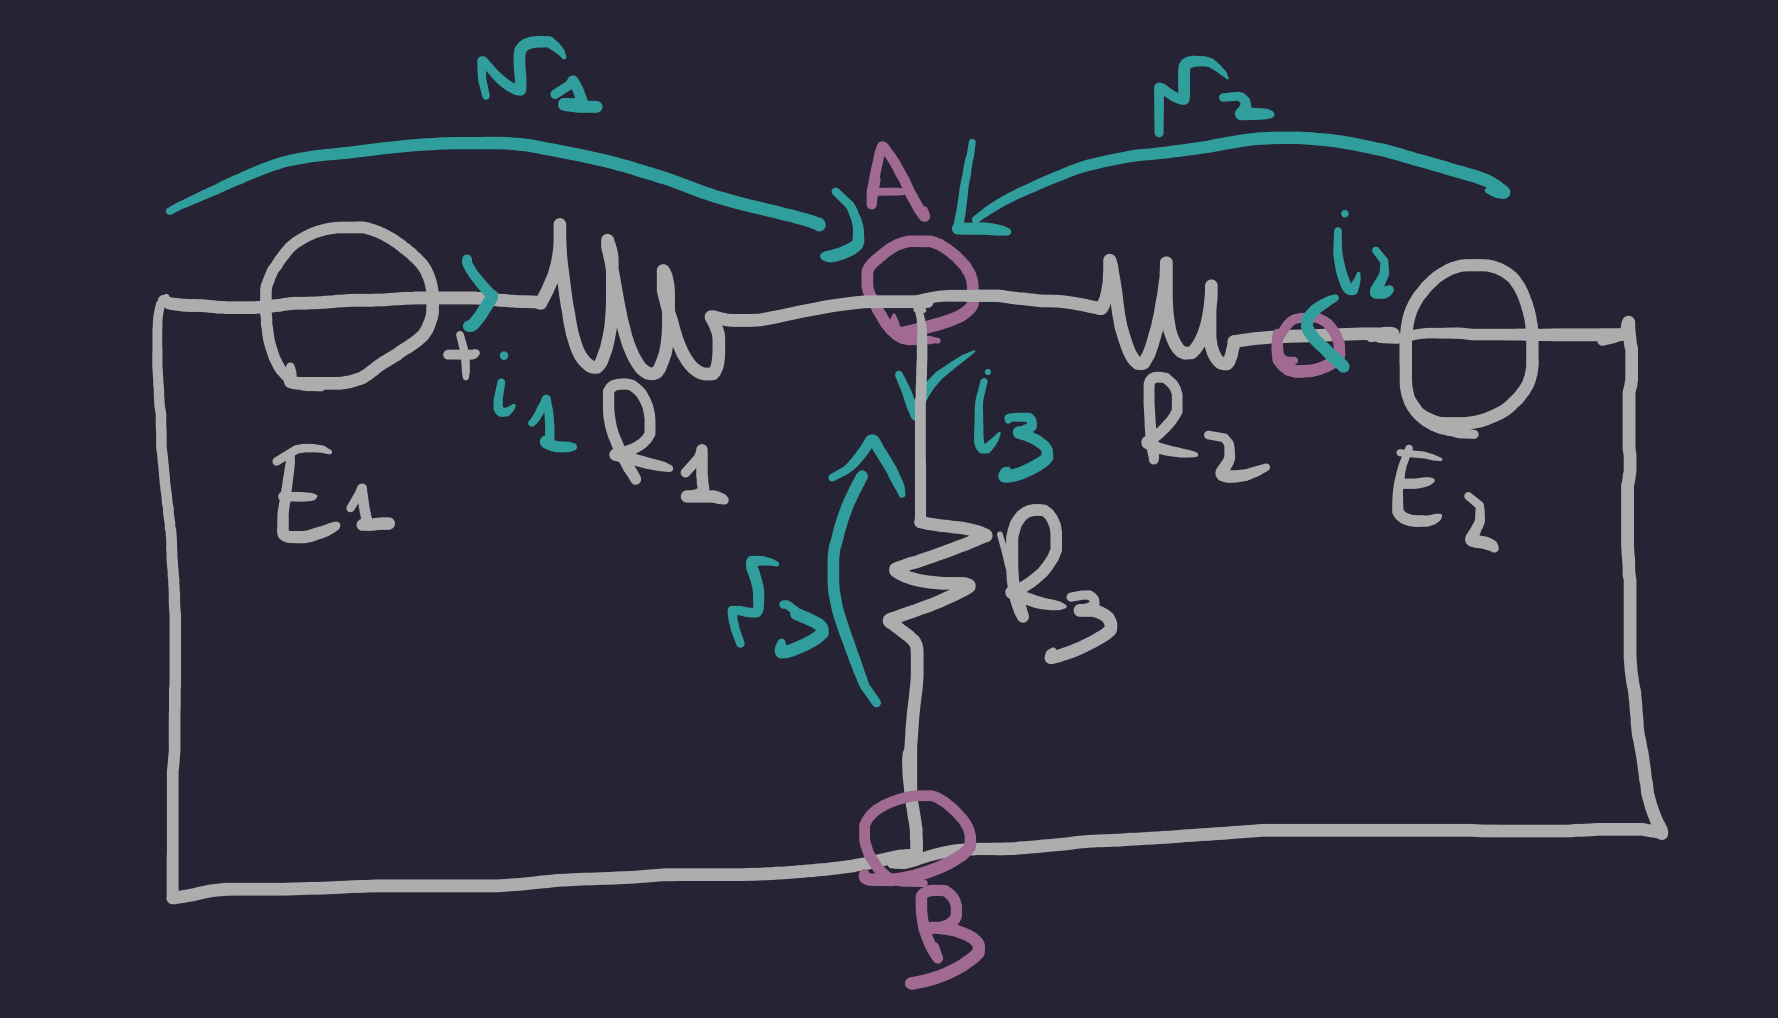
\includegraphics[scale=0.2]{Image/Esempio_MetAnalisi_1.png}
\end{center}
Calcoliamo $i_3$.\\
Bisogna considerare una causa alla volta, quindi passivare alcuni generatori: passivando un \underline{generatore di tensione} si ottiene un corto-circuito (quindi il circuito è chiuso), mentre se si passiva un generatore di corrente il circuito risultante è aperto. Per calcolare $v_3$ utilizzeremo la formula del partitore di tensione.
\subsubsection*{Causa \texorpdfstring{$E_1$}{E1}}
\begin{center}
    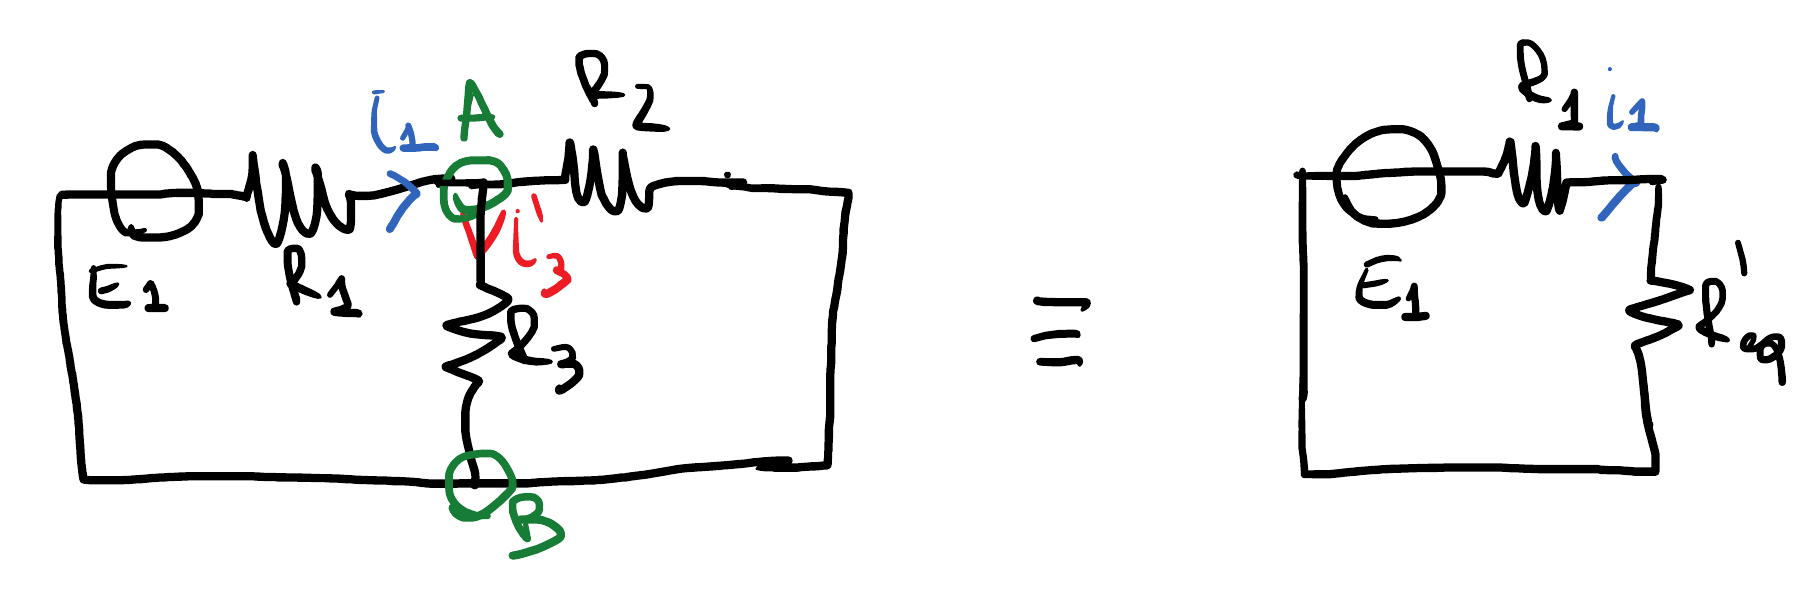
\includegraphics[scale=0.3]{Image/Esempio_MetAnal_2.png}
\end{center}

\begin{align*}
    &i_3' = i_1 \cdot \dfrac{R_2}{R_2 + R_3} = \dfrac{E_1}{R_1 + R_{eq}'} \cdot \dfrac{R_2}{R_2 + R_3} 
    & i_1 = \dfrac{E_1}{R_1 + R_{eq}'}\\
    &R_{eq}' = R_2 // R_3 = \dfrac{R_2 \cdot R_3}{R_2 + R_3} 
\end{align*}

Calcoli alternativi (più espliciti):
\begin{align*}
    &i_1 = \dfrac{E_1}{R_1 + R_{eq}'} & &v_3= \frac{R_{eq}'}{R_1+R_{eq}'} \cdot E_1 = \frac{R_2 \cdot R_3}{R_2+R_3} \cdot \frac{E_1}{R_1+R_{eq}'} =
    \frac{R_2 \cdot R_3}{R_2+R_3} \cdot i_1 \\
    &R_{eq}' = R_2 // R_3 = \dfrac{R_2 \cdot R_3}{R_2 + R_3} &
    &i_3' = \frac{v_3}{R_3} = \frac{R_2}{R_2+R_3} \cdot i_1
\end{align*}

\subsubsection*{Causa \texorpdfstring{$E_2$}{E2}}
\begin{center}
    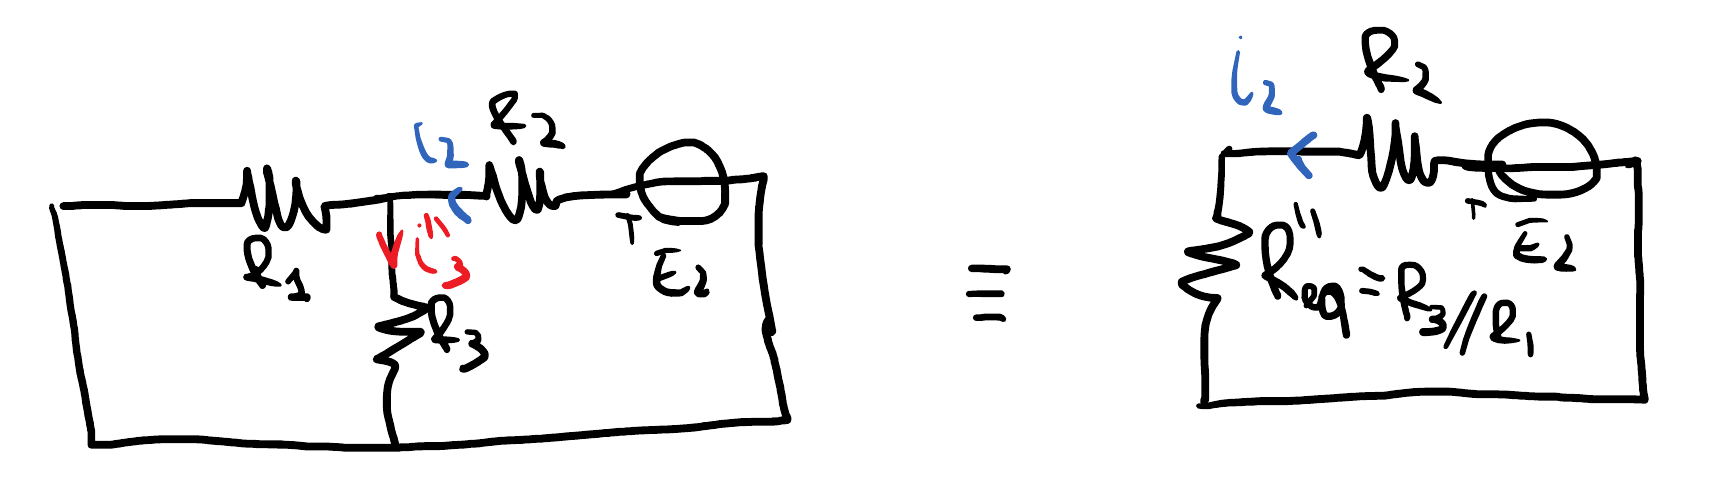
\includegraphics[scale=0.25]{Image/Esempio_MetAnalisi_3.png}
\end{center}
\begin{align*}
    &i_2 = \dfrac{E_2}{R_2+R_{eq}'} & &i_3'' = i_2 \cdot \dfrac{R_1}{R_1+R_3}
\end{align*}

Calcoli alternativi (più espliciti):
\begin{align*}
    &i_2=\frac{E_2}{R_2+R_{eq}''} & 
    &v_3 = \frac{R_{eq}''}{R_2+R_{eq}''} \cdot E_2 = \frac{R_1 \cdot R_3}{R_1+R_3} \cdot \frac{E_2}{R_2+R_{eq}''} = \frac{R_1 \cdot R_3}{R_1+R_3} \cdot i_2 \\
    &R_{eq}'' = \frac{R_1 \cdot R_3}{R_1+R_3} &
    &i_3'' = \frac{v_3}{R_3} = \frac{R_1}{R_1+R_3} \cdot i_2 
\end{align*}

Ora possiamo calcolare $i_3$:
\[
    i_3 = i_3' + i_3''
\]

\subsubsection{Esempio 2}
\begin{center}
    \includegraphics[scale=0.3]{Image/Esempio_MetAnalisi_4.png}
\end{center}
\begin{align*}
    &I'= \dfrac{E}{R} & &I'' = - \dfrac{E}{R}
\end{align*}
\begin{align*}
    &I = I' + I'' = \dfrac{E}{R} - \dfrac{E}{R} = 0 & &P=RI^2 = 0
\end{align*}
\begin{align*}
    P &= P' + P'' \\
    &= R (I')^2 + R(I'')^2 \\
    &= R \left( \dfrac{E}{R}\right)^2 + R \left(- \dfrac{E}{R}\right)^2\\
    &=R \dfrac{E^2}{R^2} + R \dfrac{E^2}{R^2} \neq 0
\end{align*}








\subsection{Teorema di Thevenin}
In un circuito lineare tempo-indipendente è messa in evidenza una porta. Il circuito N visto dalla porta, è equivalente ad un circuito formato dalla serie di un generatore indipendente di tensione ed un resistore. La tensione del generatore è data dalla tensione a vuoto
della porta AB del circuito N. Il resistore è il resistore equivalente di N visto dalla porta AB quando tutti i generatori indipendenti interni al circuito N sono spenti.
\vspace*{0.2cm}\\
Ipotesi:
\begin{itemize}
    \item circuito lineare
    \item il carico non è accoppiato con la rete da semplificare
\end{itemize}
\begin{center}
    \includegraphics[scale=0.3]{Image/Thevenin_1.png}
    \includegraphics[scale=0.3]{Image/Thevenin_2.png}
\end{center}
$E_{eq}$ è la tensione vista ai morsetti A e B a circuito aperto.\\
$R_{eq}$ è la resistenza equivalente vista da A e B passivando i generatori indipendenti.


\subsubsection{Esempio}
\begin{center}
    \includegraphics[scale=0.27]{Image/Esempio_Thevenin_1.png}
\end{center}
Applichiamo il teorema di Thevenin ai morsetti A e B:
\begin{center}
    \includegraphics[scale=0.3]{Image/Esempio_Thevenin_2.png}
\end{center}
Utilizzando l'LKT sulla maglia più grande:
\begin{align*}
    E_1 - v_{R_1} + v_{R_2} - E_2=0 &\Rightarrow E_1 - R_1i - R_2i - E_2=0\\
    &\Rightarrow E_1 - E_2 = R_1i + R_2 i \\
    & \Rightarrow E_1 - E_2 = (R_1 + R_2)i\\ 
    & \Rightarrow i = \frac{E_1-E_2}{R_1+R_2}
\end{align*}
mentre l'LKT sulla maglia più piccola a sinistra:
\begin{align*}
    E_1 - R_1i -E_{eq}=0 \underbrace{\Rightarrow}_{i=\frac{E_1-E_2}{R_1+R_2}} E_{eq} &= E-R_1 \cdot \frac{E_1-E_2}{R_1+R_2} \\
    &= \frac{\cancel{E_1R_1}+E_1R_2-\cancel{R_1E_1}+R_1E_2}{R_1+R_2}\\
    & = \frac{E_1R_2+E_2R_1}{R_1+R_2}
\end{align*}
\begin{center}
    \includegraphics[scale=0.28]{Image/Esempio_Thevenin_3.png}
\end{center}
\[
    R_{eq} = R_1 // R_2 = \frac{R_1 \cdot R_2}{R_1 + R_2}
\]
\begin{center}
    \includegraphics[scale=0.27]{Image/Esempio_Thevenin_4.png}
\end{center}
\[
    i_3 = \frac{E_{eq}}{R_3+R_{eq}} = \frac{E_1R_2+E_2R_1}{R_1+R_2} \cdot \frac{1}{R_3+R_{eq}}
\]


\subsubsection{Esercizio}
Si consideri il seguente circuito:
\begin{center}
    \includegraphics[scale=0.33]{Image/Esercizio_Thevenin_1.png}
\end{center}
Vogliamo calcolare la corrente nella resistenza $R_5$; utilizzando il teorema di Thevenin otteniamo il circuito
\begin{center}
    \includegraphics[scale=0.33]{Image/Esercizio_Thevenin_2.png}
\end{center}
e il circuito della $R_{eq}$ è il seguente
\begin{center}
    \includegraphics[scale=0.33]{Image/Esercizio_Thevenin_3.png}
\end{center}
Da notare che le resistenze $R_1$ e $R_2$ (come anche $R_3$ e $R_4$) sono in serie viste da B e C, cosa non vera nel circuito ottenuto corto-circuitando la resistenza $R_5$.
\[
    R_{eq} = (R_1+R_2) // (R_3+R_4)
\]
\begin{center}
    \includegraphics[scale=0.3]{Image/Esercizio_Thevenin_4.png}
\end{center}
Per calcolare $E_{eq}$ consideriamo la maglia $M_1$ nel circuito ottenuto corto-circuitando la resistenza $R_5$; è evidente che $e_B$ è concorde a essa, mentre $e_C$ è discorde, quindi (chiamando la tensione del circuito aperto $E_{CA}$)
\begin{align*}
    M_1: e_B - E_{CA} - e_C= 0 \Longrightarrow E_{CA} &= e_B - e_C\\
    &= R_2I_2 - R_4I_3\\
    &=R_2 \dfrac{E}{R_1+R_2} - R_4 \dfrac{E}{R_3+R_4} = E_{eq}
\end{align*}
\[
    I_5 = \frac{E_{eq}}{R_{eq}+R_5}
\]





\subsection{Teorema di Norton}
In un circuito N lineare tempo-indipendente è messa in evidenza una porta. Visto dalla porta
il circuito è equivalente ad un circuito formato dal parallelo di un generatore indipendente di
corrente ed un resistore. La corrente del generatore è data dalla corrente di cortocircuito della porta AB del circuito N. Il resistore è il resistore equivalente di N visto dalla porta AB quando tutti i generatori indipendenti interni al circuito N sono spenti.
\begin{center}
    \includegraphics[scale=0.3]{Image/Norton_1.png}
    \includegraphics[scale=0.3]{Image/Norton_2.png}
\end{center}
Ipotesi:
\begin{itemize}
    \item circuito lineare
    \item il carico non è accoppiato con la rete da semplificare
\end{itemize}
$I_{eq}$ è la corrente tra A e B quando vi è un corto-circuito.\\
$R_{eq}$ è resistenza vista ai morsetti A e B passivando i generatori indipendenti.


\subsubsection{Esempio}
\begin{center}
    \includegraphics[scale=0.25]{Image/Esempio_Norton_0.png}
\end{center}
Vogliamo calcolare $i_3$. Quindi applichiamo il teorema di Norton, utilizzando la formula del partitore di corrente per calcolare $i_3$:
\begin{center}
    \begin{tabular}{c c c}
        \includegraphics[scale=0.25]{Image/Esempio_Norton_1.png}&\includegraphics[scale=0.25]{Image/Esempio_Norton_2.png} & \includegraphics[scale=0.25]{Image/Esempio_Norton_3.png}\\
        $I_{eq} = i_1+i_2 = \dfrac{E_1}{R_1} + \dfrac{E_2}{R_2}$ & $R_{eq} = R_1 // R_2 = \dfrac{R_1 \cdot R_2}{R_1+R_2}$ & $i_3 = I_{eq} \cdot \dfrac{R_{eq}}{R_{eq}+R_3}$
    \end{tabular}
\end{center}





\subsection{Teorema del massimo trasferimento di potenza}
Consideriamo il seguente circuito
\begin{center}
    \includegraphics[scale=0.3]{Image/T_Massima_Potenza_0.png}
\end{center}
Qual è il valore di $R_L$ che massimizza il trasferimento di potenza? Proviamo a calcolarlo.
\begin{align*}
    P_L &= I \cdot V_L\\
    &=R_L \cdot I^2\\
    &=R_L \left( \dfrac{E}{R+R_L} \right)^2 
    \begin{cases}
        R_L=0 \Rightarrow P_L=0\\
        R_L \rightarrow \infty \Rightarrow P_L=0 \text{ (circuito aperto)}
    \end{cases}
\end{align*}
\begin{center}
    \includegraphics[scale=0.25]{Image/T_Massima_Potenza_1.png}
\end{center}
Per trovare il massimo poniamo la derivata della potenza a 0; sapendo che $P_L = E^2 \dfrac{R_L}{(R+R_L)^2}$
\begin{align*}
    \dfrac{\partial P_L}{\partial R_L}=0 &\Rightarrow E^2 \dfrac{(R+R_L)^2 - 2R_L(R+R_L)}{(R+R_L)^4}=0\\
    & \Rightarrow R^2 + \cancel{R^2_L} + \cancel{2RR_L} - \cancel{2RR_L} -\cancel{2}R^2_L = 0\\
    &\Rightarrow R=R_L
\end{align*} 
\begin{align*}
    P_{L,Max} &= R \dfrac{E^2}{(R+R)^2}\\
    &= \cancel{R} \dfrac{E^2}{4R^{\cancel{2}}}\\
    &= \dfrac{E^2}{4R}
\end{align*}



\subsection{Teorema di Millman}
Data una rete con due o più lati in parallelo, la tensione ai capi della rete è pari al rapporto delle correnti di corto-circuito di ogni singolo lato e la sommatoria delle conduttanze di ogni lato.
\begin{center}
    \includegraphics[scale=0.26]{Image/Th_Millman_0.png}
\end{center}
\[
    v_{AB} = \frac{\sum\limits_k \frac{v_k}{R_k} + \sum\limits_j i_j}{\sum\limits_n\frac{1}{R_n}}
\]

\subsubsection{Esempio 1}
\begin{center}
    \includegraphics[scale=0.25]{Image/Es_Millman.png}
\end{center}
\[
    v_{AB} =\frac{\frac{E_1}{R_1}+\frac{E_2}{R_2} + I_3}{\frac{1}{R_1}+\frac{1}{R_2}+\frac{1}{R_3}}
\]
Dimostriamo che questa formula è vera utilizzando il metodo dei potenziali di nodo (applicato al nodo B):
\begin{center}
    \includegraphics[scale=0.3]{Image/Dim_Es_Millman.png}
\end{center}
\begin{align}
    &v_{AB} = E_1 - R_1i_1 \Rightarrow i_1 = \frac{E_1-v_{AB}}{R_1}\\
    &v_{AB} = -E_2+R_2i_2 \Rightarrow i_2 = \frac{E_2+v_{AB}}{R_2}    \\
    &i_3 = I_3    \\
    &i_4 = \frac{v_{AB}}{R_4}
\end{align}
\begin{align*}
    \text{LKC: } i_1-i_2+i_3-i_4=0 &\Rightarrow \frac{E_1-v_{AB}}{R_1} - \frac{E_2+v_{AB}}{R_2} + I_3 - \frac{v_{AB}}{R_4} = 0\\
    &\Rightarrow \frac{E_1}{R_1} - \frac{v_{AB}}{R_1} - \frac{E_2}{R_2} - \frac{v_{AB}}{R_2} + I_3 - \frac{v_{AB}}{R_4} = 0\\
    &\Rightarrow v_{AB} \left( \frac{1}{R_1} + \frac{1}{R_2} + \frac{1}{R_3} \right) = \frac{E_1}{R_1} - \frac{E_2}{R_2} + I_3\\
    &\Rightarrow v_{AB} = \frac{\frac{E_1}{R_1}+\frac{E_2}{R_2} + I_3}{\frac{1}{R_1}+\frac{1}{R_2}+\frac{1}{R_3}}
\end{align*}

\subsubsection{Esempio 2}
\begin{center}
    \includegraphics[scale=0.3]{Image/Es_Millman_2.png}
\end{center}
Calcoliamo $i_3$:
\[
    v_{AB} = \frac{\frac{E_1}{R_1}+\frac{E_2}{R_2}}{\frac{1}{R_1}+\frac{1}{R_2}+\frac{1}{R_3}} \Rightarrow i_3 = \frac{v_{AB}}{R_3}
\]























\end{document}